%!TEX encoding = UTF-8 Unicode
\documentclass{lecturehandouts}

\setbeamertemplate{footline}[frame number]
\title[Föreläsningsanteckningar pgk, 2016]{Programmering, grundkurs \code{pgk}}
\subtitle{Föreläsningsanteckningar \code{pgk} (EDAA45)}
\author{Björn Regnell}
\institute{Datavetenskap, LTH}
\date{Lp1-2, HT 2016}

\setbeamerfont{section in toc}{size=\small}

\setbeamerfont{subsection in toc}{size=\footnotesize}

\begin{document}

%\renewcommand{\pause}{}
%!TEX encoding = UTF-8 Unicode
\newcommand{\ExeWeekONE}{expressions}
\newcommand{\LabWeekONE}{kojo}

\newcommand{\ExeWeekTWO}{programs}
\newcommand{\LabWeekTWO}{--}

\newcommand{\ExeWeekTHREE}{functions}
\newcommand{\LabWeekTHREE}{blockmole}

\newcommand{\ExeWeekFOUR}{data}
\newcommand{\LabWeekFOUR}{pirates}

\newcommand{\ExeWeekFIVE}{sequences}
\newcommand{\LabWeekFIVE}{shuffle}

\newcommand{\ExeWeekSIX}{classes}
\newcommand{\LabWeekSIX}{turtlegraphics}

\newcommand{\ExeWeekSEVEN}{traits}
\newcommand{\LabWeekSEVEN}{turtlerace-team}

\newcommand{\ExeWeekEIGHT}{matching}
\newcommand{\LabWeekEIGHT}{chords-team}

\newcommand{\ExeWeekNINE}{matrices}
\newcommand{\LabWeekNINE}{maze}

\newcommand{\ExeWeekTEN}{sorting}
\newcommand{\LabWeekTEN}{survey}

\newcommand{\ExeWeekELEVEN}{scalajava}
\newcommand{\LabWeekELEVEN}{lthopoly-team}

\newcommand{\ExeWeekTWELVE}{threads}
\newcommand{\LabWeekTWELVE}{life}

\newcommand{\ExeWeekTHIRTEEN}{Uppsamling}
\newcommand{\LabWeekTHIRTEEN}{Projekt}

\newcommand{\ExeWeekFOURTEEN}{Extenta}
\newcommand{\LabWeekFOURTEEN}{--}



\newcommand{\Lecture}[2]{%
\section[Vecka #1: #2]{#2}%
\frame{\tableofcontents[currentsubsection,hideothersubsections,sections={#1}]}}

\frame{\titlepage}
\frame{
\vspace{-1em}\begin{multicols}{2}
\tableofcontents[subsectionstyle=hide,sections={1-7}]

\columnbreak

\tableofcontents[subsectionstyle=hide,sections={8-14}]
\end{multicols}
}

\Lecture{1}{Introduktion}
\input{body/lect-w01-about.tex}
\input{body/lect-w01-intro.tex}

\Lecture{2}{Kodstrukturer}
%!TEX encoding = UTF-8 Unicode
%!TEX root = ../lect-w02.tex

\Subsection{Datastrukturer och kontrollstrukturer}

\begin{Slide}{Vad är en datastruktur?}\SlideFontSmall
\begin{itemize}
\item En \href{https://sv.wikipedia.org/wiki/Datastruktur}{datastruktur} är en struktur för organisering av data som...
\begin{itemize}\SlideFontTiny
\item kan innehålla \Alert{många} element,
\item kan refereras till som en helhet, och
\item ger möjlighet att komma åt enskilda element.
\end{itemize}

\item En \Emph{samling} \Eng{collection} är en datastruktur som kan innehålla många element av \Alert{samma typ}.

\item Exempel på olika samlingar där elementen är organiserade på olika vis: \\
\vspace{0.5em}
\begin{tabular}{l c}
\Emph{Lista} & \includegraphics[width=5cm]{../img/list.pdf} \\
\Emph{Träd}  & \includegraphics[width=2.2cm]{../img/tree.pdf} \\
\Emph{Graf}  & \includegraphics[width=2.2cm]{../img/graph.pdf} \\
\end{tabular}
\end{itemize}
{
\SlideFontTiny \vspace{1em }\hskip2em
Mer om listor \& träd \href{http://cs.lth.se/edaa01vt}{fördjupningskursen}.
Mer om träd, grafer i \href{http://cs.lth.se/edaa40}{Diskreta strukturer.}
}

\end{Slide}


\begin{Slide}{Vad är en vektor?}\SlideFontSmall
En \Emph{vektor}\footnote{Vektor kallas ibland på svenska även \href{https://sv.wikipedia.org/wiki/F\%C3\%A4lt_\%28datastruktur\%29}{fält}, men det skapar stor förvirring eftersom det engelska ordet \emph{field} ofta används för \emph{attribut} (förklaras senare).}
\Eng{vector, \href{https://en.wikipedia.org/wiki/Array_data_structure}{array}} är en \Emph{samling} som är \Alert{snabb} att \Emph{indexera} i.
Åtkomst av element sker med \code{apply(platsnummer)}:

\begin{REPL}
scala> val heltal = Vector(42, 13, -1, 0, 1)
heltal: scala.collection.immutable.Vector[Int] = Vector(42, 13, -1, 0, 1)

scala> heltal.apply(0)
res0: Int = 42

scala> heltal(1)    // man kan skippa .apply före (
res1: Int = 13

scala> heltal(5)
java.lang.IndexOutOfBoundsException: 5
  at scala.collection.immutable.Vector.checkRangeConvert(Vector.scala:132)
\end{REPL}
Utelämnar du \code{.apply} så skapar kompilatorn automatiskt ett anrop av \code{apply}.
\end{Slide}

\begin{Slide}{En konceptuell bild av en vektor}

\begin{REPLnonum}
scala> val heltal = Vector(42, 13, -1, 0, 1)

scala> heltal(0)
res0: Int = 42
\end{REPLnonum}

\begin{tikzpicture}[font=\ttfamily]
\matrix [matrix of nodes, row sep=0, column 2/.style={nodes={rectangle,draw,minimum width=3em}}] (var) at (0cm, 2.8cm)
{
heltal   &  \makebox(16,12){ }\\
};
\matrix [matrix of nodes, draw=black,row sep=0, column 2/.style={nodes={rectangle,draw,minimum width=4em}}] (vec) at (4cm, 1cm)
{
\textit{plats} &  \\
0   &  \makebox(16,12){42}\\
1   &  \makebox(16,12){13}\\
2   &  \makebox(16,12){-1}\\
3   &  \makebox(16,12){0}\\
4   &  \makebox(16,12){1}\\
};
\filldraw[black] (0.7cm,2.8cm) circle (3pt) node[] (ref) {};
 \draw [arrow] (ref) -- (vec);
\end{tikzpicture}

%\vspace{1em} Elementen ligger på rad någonstans i minnet.
\end{Slide}



\begin{Slide}{En samling strängar}

\begin{itemize}
\item En vektor kan lagra många värden av samma typ.
\item Elementen kan vara till exempel heltal eller strängar.
\item Eller faktiskt vad som helst. (En s.k. \emph{generisk} samling.)
\end{itemize}

\begin{REPL}
scala> val grönsaker = Vector("gurka","tomat","paprika","selleri")
grönsaker: scala.collection.immutable.Vector[String] =
  Vector(gurka, tomat, paprika, selleri)

scala> val g = grönsaker(1)
g: String = tomat

scala> val xs = Vector(42, "gurka", true, 42.0)
xs: scala.collection.immutable.Vector[Any] = Vector(42, gurka, true, 42.0)
\end{REPL}
Notera typen \code{Any} (mer om denna typ senare).
\end{Slide}

\begin{Slide}{Vad är en kontrollstruktur?}
\begin{itemize}
\item En \Emph{kontrollstruktur} påverkar \Alert{sekvensen}.
\begin{itemize}
\item[] Exempel på inbyggda kontrollstrukturer:
\\\vspace{0.5em}\code{for}-sats, \code{while}-sats
\end{itemize}

\item[]

\item I Scala kan man definiera \Emph{egna} kontrollstrukturer.
\begin{itemize}
\item[] Exempel: \code{upprepa} som du använt i Kojo
\\\vspace{0.5em}\code|upprepa(4){fram; höger}|
\end{itemize}
\end{itemize}
\end{Slide}

\ifkompendium\else
\begin{Slide}{Mitt första program: en oändlig loop på ABC80}
\begin{minipage}{0.8\textwidth}
\begin{verbatim}
10 print "hej"
20 goto 10
\end{verbatim}
\includegraphics[width=0.8\textwidth]{../img/abc80.jpg}
\end{minipage}%
\begin{minipage}{0.2\textwidth}
\pause
\begin{verbatim}
hej
hej
hej
hej
hej
hej
hej
hej
hej
hej
hej
hej
<Ctrl+C>
\end{verbatim}
\end{minipage}
\end{Slide}
\fi

\begin{Slide}{Loopa genom elementen i en vektor}
En \code{for}-\Emph{sats} som skriver ut alla element i en vektor:
\begin{REPL}
scala> val grönsaker = Vector("gurka","tomat","paprika","selleri")

scala> for (g <- grönsaker) println(g)
gurka
tomat
paprika
selleri

\end{REPL}

\end{Slide}


\begin{Slide}{Bygga en ny samling från en befintlig med for-uttryck}
Ett \code{for}-\code{yield}-\Emph{uttryck} som \Emph{skapar en \Alert{ny} samling}.

\begin{Code}[basicstyle=\ttfamily\fontsize{12}{14}\selectfont]
for (g <- grönsaker) yield "god " + g
\end{Code}

\begin{REPL}
scala> val grönsaker = Vector("gurka","tomat","paprika","selleri")

scala> for (g <- grönsaker) yield "god " + g
res0: scala.collection.immutable.Vector[String] =
  Vector(god gurka, god tomat, god paprika, god selleri)

scala> val åsikter = for (g <- grönsaker) yield s"god $g"
åsikter: scala.collection.immutable.Vector[String] =
  Vector(god gurka, god tomat, god paprika, god selleri)
\end{REPL}

\end{Slide}


\begin{Slide}{Samlingen \code{Range} håller reda på intervall}
\begin{itemize}
\item Med en \code{Range(start, slut)} kan du skapa ett intervall: \\ från och med \code{start} till (men inte med) \code{slut}
\end{itemize}

\begin{REPLnonum}
scala> Range(0, 42)
res0: scala.collection.immutable.Range =
  Range(0, 1, 2, 3, 4, 5, 6, 7, 8, 9, 10, 11, 12, 13, 14,
    15, 16, 17, 18, 19, 20, 21, 22, 23, 24, 25, 26, 27, 28,
    29, 30, 31, 32, 33, 34, 35, 36, 37, 38, 39, 40, 41)
\end{REPLnonum}

\begin{itemize}
\item Men alla värden däremellan skapas inte förrän de behövs:
\end{itemize}

\begin{REPL}
scala> val jättestortIntervall = Range(0, Int.MaxValue)
jättestortIntervall: scala.collection.immutable.Range = Range(0, 1, 2, 3, 4, 5, ...

scala> jättestortIntervall.end
res1: Int = 2147483647

scala> jättestortIntervall.toVector
java.lang.OutOfMemoryError: GC overhead limit exceeded
\end{REPL}

\end{Slide}

\begin{Slide}{Loopa med Range}
\code{Range} används i for-lopar för att hålla reda på antalet rundor.
\begin{REPLnonum}
scala> for (i <- Range(0, 6)) print(" gurka " + i)
 gurka 0 gurka 1 gurka 2 gurka 3 gurka 4 gurka 5
\end{REPLnonum}
Du kan skapa en \code{Range} med \code{until} efter ett heltal:
\begin{REPLnonum}
scala> 1 until 7
res1: scala.collection.immutable.Range =
  Range(1, 2, 3, 4, 5, 6)

scala> for (i <- 1 until 7) print(" tomat " + i)
 tomat 1 tomat 2 tomat 3 tomat 4 tomat 5 tomat 6

\end{REPLnonum}
\end{Slide}

\begin{Slide}{Loopa med Range skapad med \texttt{to}}

Med \code{to} efter ett heltal får du en \code{Range} till och \Emph{med} sista:
\begin{REPLnonum}
scala> 1 to 6
res2: scala.collection.immutable.Range.Inclusive =
  Range(1, 2, 3, 4, 5, 6)

scala> for (i <- 1 to 6) print(" gurka " + i)
 gurka 1 gurka 2 gurka 3 gurka 4 gurka 5 gurka 6

\end{REPLnonum}


\end{Slide}



\begin{Slide}{Vad är en \code{Array} i JVM?}


\begin{itemize}
\item En \code{Array} liknar en \code{Vector} men har en särställning i JVM:
\begin{itemize}
\item Lagras som en sekvens i minnet på efterföljande adresser.
\item \Emph{Fördel}: snabbaste samlingen för element-access i JVM.
\item Men det finns en hel del \Alert{nackdelar} som vi ska se senare.
\end{itemize}

\end{itemize}

\begin{REPLnonum}
scala> val heltal = Array(42, 13, -1, 0 , 1)
\end{REPLnonum}

\begin{tikzpicture}[font=\ttfamily,scale=0.75, every node/.style={scale=0.75}]
\matrix [matrix of nodes, row sep=0, column 2/.style={nodes={rectangle,draw,minimum width=3em}}] (var) at (0cm, 2.8cm)
{
heltal   &  \makebox(16,12){ }\\
};
\matrix [matrix of nodes, draw=black,row sep=0, column 2/.style={nodes={rectangle,draw,minimum width=4em}}] (vec) at (4cm, 1cm)
{
\textit{plats} &  \\
0   &  \makebox(16,12){42}\\
1   &  \makebox(16,12){13}\\
2   &  \makebox(16,12){-1}\\
3   &  \makebox(16,12){0}\\
4   &  \makebox(16,12){1}\\
};
\filldraw[black] (0.7cm,2.8cm) circle (3pt) node[] (ref) {};
 \draw [arrow] (ref) -- (vec);
\end{tikzpicture}
\end{Slide}

\begin{Slide}{Några likheter \& skillnader mellan \texttt{Vector} och \texttt{Array}}\SlideFontSmall
\begin{multicols}{2}
\begin{REPLnonum}
scala> val xs = Vector(1,2,3)
\end{REPLnonum}

\columnbreak

\begin{REPLnonum}
scala> val xs = Array(1,2,3)
\end{REPLnonum}
\end{multicols}


Några likheter mellan \texttt{Vector} och \texttt{Array}
\begin{itemize}
\item Båda är samlingar som kan innehålla många element.

\item Med båda kan man snabbt accessa vilket element som helst: \code{xs(2)}
\end{itemize}
Några viktiga skillnader:

\vspace{-0.5em}\begin{multicols}{2}
\Emph{Vector}
\begin{itemize}
\item Är \Emph{oföränderlig}: du kan lita på att elementreferenserna aldrig någonsin kommer att ändras.

\item Är \Emph{snabb på att skapa en delvis förändrad kopia}, t.ex. tillägg/borttagning/uppdatering mitt i sekvensen.

\end{itemize}


\columnbreak

\Alert{Array}
\begin{itemize}
\item Är \Alert{föränderlig}: \code{xs(2) = 42}

\item Är \Alert{snabb} om man bara vill läsa eller skriva på befintliga platser.

\item Är \Alert{långsam} om man vill lägga till eller ta bort element mitt i sekvensen.
\item Kan \Alert{ej} ändra storlek.

\end{itemize}
\end{multicols}
\end{Slide}



\Subsection{Huvudprogram med \texttt{main} i Scala och Java}

\begin{Slide}{Ett minimalt fristående program i Scala och Java}
Nedan Scala-kod skrivs i en editor, spara med valfritt filnamn:
\begin{Code}
// this is Scala

object Hello {
  def main(args: Array[String]): Unit = {
    println("Hejsan scala-appen!")
  }
}
\end{Code}

\pause
\vspace{1em}
Nedan Java-kod skrivs i en editor, filen \Alert{måste} heta \texttt{Hi.java}

\begin{Code}[language=Java]
// this is Java

public class Hi {
    public static void main(String[] args) {
        System.out.println("Hejsan Java-appen!");
    }
}
\end{Code}

\end{Slide}


\begin{Slide}{Loopa genom en samling med en \texttt{while}-sats}
\begin{REPLnonum}
scala> val xs = Vector("Hej","på","dej","!!!")
xs: scala.collection.immutable.Vector[String] =
  Vector(Hej, på, dej, !!!)

scala> xs.size
res0: Int = 4

scala> var i = 0
i: Int = 0

scala> while (i < xs.size) { println(xs(i)); i = i + 1 }
Hej
på
dej
!!!
\end{REPLnonum}
\end{Slide}


\begin{Slide}{Loopa genom argumenten i ett Scala-huvudprogram}
Skriv denna kod och spara i filen \texttt{helloargs.scala}
\begin{REPLnonum}
$ gedit helloargs.scala
\end{REPLnonum}
\begin{Code}
object HelloScalaArgs {
  def main(args: Array[String]): Unit = {
    var i = 0
    while (i < args.size) {
      println(args(i))
      i = i + 1
    }
  }
}
\end{Code}
Kompilera och kör:
\begin{REPL}
$ scalac helloargs.scala
$ scala HelloScalaArgs hej gurka tomat
hej
gurka
tomat
\end{REPL}
\end{Slide}


\begin{Slide}{Loopa genom argumenten i ett Java-huvudprogram}
\begin{REPLnonum}
$ gedit HelloJavaArgs.java
\end{REPLnonum}
\begin{Code}[language=Java]
// this is Java

public class HelloJavaArgs {
    public static void main(String[] args) {
    int i = 0;
    while (i < args.length) {
      System.out.println(args[i]);
      i = i + 1;
    }
  }
}
\end{Code}
Kompilera och kör:
\begin{REPL}
$ javac HelloJavaArgs.java
$ java HelloJavaArgs hej gurka tomat
hej
gurka
tomat
\end{REPL}

\end{Slide}


\begin{Slide}{Scala-skript}
\begin{itemize}
\item Skala-kod kan köras som ett \Emph{skript}.\footnote{\SlideFontTiny Du får prova detta på övningen. Vi kommer mest att köra kompilerat i kursen, då Scala-skript saknar mekanism för inkludering av andra skript. Men det finns ett öppenkällkodsprojekt som löser det: \url{http://www.lihaoyi.com/Ammonite/}
}
\item Ett skript kompileras varje gång innan det körs och maskinkoden sparas inte som vid vanlig kompilering.
\item Då behövs ingen \code{main} och inget \code{object}
\end{itemize}

\begin{Code}[basicstyle=\ttfamily\fontsize{10}{12}\selectfont]
// spara nedan i filen 'myscript.scala'

println("Hejsan argumnet!")
for (arg <- args) println(arg)
\end{Code}

\begin{REPLnonum}
$ scala myscript.scala
\end{REPLnonum}


\end{Slide}



\Subsection{Algoritmer: stegvisa lösningar}

\begin{Slide}{Vad är en algoritm?}
En \href{https://sv.wikipedia.org/wiki/Algoritm}{algoritm} är en sekvens av instruktioner som beskriver \\hur man löser ett problem.\\
\vspace{1em}
\Emph{Exempel}:
\begin{itemize}
\item	 baka en kaka
\pause\item räkna ut din pensionsprognos
\pause\item köra bil
\pause\item kolla om highscore i ett spel
\item ...
\end{itemize}

\begin{tikzpicture}[overlay]
\node[xshift=0.85\textwidth, scale=2.0] { \includegraphics[width=0.25\textwidth]{../img/highscore}};
\end{tikzpicture}
\end{Slide}


\ifkompendium\else
\begin{Slide}{Algoritm-exempel: HIGHSCORE}
\Emph{Problem}: Kolla om high-score i ett spel \\ \vspace{1em}

\Emph{Varför?} \pause Så att de som spelar uppmuntras att spela mer :) \\ \vspace{1em}

\Emph{Algoritm:}\pause
\begin{enumerate}
\item $points$ $\leftarrow$ poängen efter senaste spelet
\item $highscore$ $\leftarrow$ bästa resultatet innan senaste spelet
\item \Key{om} $points$ är större än $highscore$
\begin{enumerate}[ ~~]
\item  Skriv ''Försök igen!''
\end{enumerate}
\Key{annars}
\begin{enumerate}[ ~~]
\item  Skriv ''Grattis!''
\end{enumerate}
\end{enumerate}
\pause
\scriptsize \Alert{Hittar du buggen?}

\pause Utskriften blir fel; vänd villkor eller byt plats på grenarna i if-satsen
\end{Slide}
\fi


\begin{Slide}{HIGHSCORE implementerad i Scala}
\begin{Code}
import scala.io.StdIn.readLine

object HighScore {
  def main(args: Array[String]): Unit = {
    val points = readLine("Hur mång poäng fick du?").toInt
    val highscore = readLine("Vad var highscore före senaste spelet?").toInt
    val msg = if (points > highscore) "GRATTIS!" else "Försök igen!"
    println(msg)
  }
}
\end{Code}
\pause
Är det en bugg eller en feature att det står\\ \texttt{points > highscore} \\ och inte \\ \texttt{points >= highscore} \\ ?
% Buggen är att man inte får GRATTIS om poäng == highscore vilket är tråkigt :)
\end{Slide}


\begin{Slide}{HIGHSCORE implementerad i Java}
\begin{Code}[language=Java]
import java.util.Scanner;

public class HighScore {
    public static void main(String[] args){
        Scanner scan = new Scanner(System.in);
        System.out.println("Hur många poäng fick du?");
        int points =  scan.nextInt();
        System.out.println("Vad var highscore före senaste spelet?");
        int highscore = scan.nextInt();
        if (points > highscore) {
            System.out.println("GRATTIS!");
        } else {
            System.out.println("Försök igen!");
        }
    }
}
\end{Code}
\end{Slide}


\begin{Slide}{Algoritmexempel: N-FAKULTET}
\begin{algorithm}[H]
 \SetKwInOut{Input}{Indata}\SetKwInOut{Output}{Resultat}

 \Input{heltalet $n$}
 \Output{utskrift av produkten av de första $n$ heltalen }
 ~\\
 $prod \leftarrow 1$ \\
 $i \leftarrow 2$  \\
 \While{$i \leq n$}{
  $prod \leftarrow prod * i$\\
  $i \leftarrow i + 1$
 }
 skriv ut $prod$
\end{algorithm}
\pause\vspace{1em}
\begin{itemize}\SlideFontSmall
\item Vad händer om $n$ är noll?
\item Vad händer om $n$ är ett?
\item Vad händer om $n$ är två?
\item Vad händer om $n$ är tre?
\end{itemize}
\end{Slide}

\begin{Slide}{Algoritmexempel: MIN}
\begin{algorithm}[H]
 \SetKwInOut{Input}{Indata}\SetKwInOut{Output}{Resultat}

 \Input{Array $args$ med strängar som alla innehåller heltal}
 \Output{utskrift av minsta heltalet }
 ~\\
 $min \leftarrow$ det största heltalet som kan uppkomma  \\
 $n \leftarrow $ antalet heltal \\
 $i \leftarrow 0$ \\
 \While{$i < n$}{
   $x \leftarrow args(i).toInt$ \\
   \If{( x < $min$)}{$min \leftarrow x$}
   $i \leftarrow i + 1$
 }
 skriv ut $min$
\end{algorithm}
\pause{\hfill \SlideFontTiny \Emph{Testa med indata}: \code{args = Array("2", "42", "1", "2")}}
\end{Slide}


\Subsection{Funktioner skapar struktur}

\begin{Slide}{Mall för funktionsdefinitioner}

\code{def} funktionsnamn(parameterdeklarationer): returtyp = block

\pause\vspace{0.5em}\Emph{Exempel}:

\begin{Code}[basicstyle=\ttfamily\fontsize{9}{11}\selectfont]
def öka(i: Int): Int = { i + 1 }
\end{Code}
\pause Om ett enda uttryck: behövs inga \code|{}|. Returtypen kan härledas.
\begin{Code}[basicstyle=\ttfamily\fontsize{9}{11}\selectfont]
def öka(i: Int) = i + 1
\end{Code}
\pause Om flera parametrar, separera dem med kommatecken:
\begin{Code}[basicstyle=\ttfamily\fontsize{9}{11}\selectfont]
def isHighscore(points: Int, high: Int): Boolean = {
  val highscore: Boolean = points > high
  if (highscore) println(":)") else print(":(")
  highscore
}
\end{Code}
\pause Ovan funktion har \Alert{sidoeffekten} att skriva ut en smiley.
\end{Slide}

\begin{Slide}{Bättre många små abstraktioner som gör en sak var}

\begin{Code}[basicstyle=\ttfamily\fontsize{8}{11}\selectfont]
def isHighscore(points: Int, high: Int): Boolean = points > high

def printSmiley(isHappy: Boolean): Unit =
  if (isHappy) println(":)") else print(":(")
\end{Code}

\pause\vspace{2em}
\begin{REPLnonum}
  printSmiley(isHighscore(113,99))
\end{REPLnonum}

\pause\vspace{2em} \code{isHighscore} är en \Emph{äkta funktion} som alltid ger samma svar för samma inparametrar och saknar \Alert{sidoeffekter}.

\end{Slide}



\begin{Slide}{Vad är ett block?}

\begin{itemize}
\item Ett block \Emph{kapslar in} flera satser/uttryck och ser ''utifrån'' ut som en enda sats/uttryck.

\item Ett block skapas med hjälp av klammerparenteser (''krullparenteser'')

\item [] {\fontsize{14}{18}\selectfont \code|{ uttryck1; uttryck2; ... uttryckN }|}\\~

\pause

\item I Scala (till skillnad från många andra språk) har ett block ett \Emph{värde} och är alltså ett \Emph{uttryck}.

\item Värdet ges av \Emph{sista uttrycket} i blocket.

\begin{REPLnonum}
scala> val x = { println(1 + 1); println(2 + 2); 3 + 3 }
2
4
x: Int = 6
\end{REPLnonum}


\end{itemize}

\end{Slide}

\begin{Slide}{Namn i block blir \textbf{lokala}}
Synlighetsregler:
\begin{enumerate}
\item Identifierare deklarerade inuti ett block blir \Emph{lokala}.

\item Lokala namn \Alert{överskuggar} namn i yttre block om samma.


\item Namn syns i nästlade underblock.

\end{enumerate}

\begin{REPL}
scala> { val lokaltNamn = 42; println(lokaltNamn) }
42

scala> println(lokaltNamn)
<console>:12: error: not found: value lokaltNamn
       println(lokaltNamn)

scala> { val x = 42; { val x = 76; println(x) }; println(x) }
76
42

scala> { val x = 42; { val y = x + 1; println(y) } }
43
\end{REPL}

\end{Slide}


\begin{Slide}{Parameter och argument}

Skilj på parameter och argument!
\begin{itemize}
\item En \Alert{parameter} är det deklarerade namnet som används \Alert{lokalt} i en funktion för att referera till...

\item \Emph{argumentet} som är värdet som skickas med \Emph{vid anrop} och binds till det lokala parameternamnet.

\end{itemize}


\begin{REPLnonum}
scala> val ettArgument = 42

scala> def öka(minParameter: Int) = minParameter + 1

scala> öka(ettArgument)
\end{REPLnonum}


Speciell syntax: anrop med s.k. \Emph{namngiven parameter}
\begin{REPLnonum}
scala> öka(minParameter = ettArgument)
\end{REPLnonum}

\end{Slide}

\begin{Slide}{Procedurer}\SlideFontSmall
\begin{itemize}
\item En \Emph{procedur} är en funktion som \Alert{gör} något intressant, men som \Alert{inte} lämnar något intressant returvärde.
\item Exempel på befintlig procedur: \code{println("hej")}
\item Du \Emph{deklarerar egna procedurer} genom att ange \texttt{\Alert{Unit}} som returvärdestyp. Då ges värdet \texttt{\Alert{()}} som betyder ''inget''.
\end{itemize}
\begin{REPL}
scala> def hej(x: String): Unit = println(s"Hej på dej $x!")
hej: (x: String)Unit

scala> hej("Herr Gurka")
Hej på dej Herr Gurka!

scala> val x = hej("Fru Tomat")
Hej på dej Fru Tomat!
x: Unit = ()
\end{REPL}
\begin{itemize}
\item Det som \Alert{görs} kallas (sido)\Emph{effekt}. Ovan är utskriften själva effekten.
\item Funktioner kan också ha sidoeffekter. De kallas då \Alert{oäkta} funktioner.
\end{itemize}
\end{Slide}

\begin{Slide}{''Ingenting'' \emph{är} faktiskt någonting i Scala}
\begin{itemize}
\item I många språk (Java, C, C++, ...) är funktioner som saknar värden speciella.
 Java m.fl. har speciell syntax för procedurer med nyckelordet \jcode{void}, men \Alert{inte} Scala.

\item I Scala är procedurer inte specialfall; de är vanliga funktioner som returnerar ett värde som \Emph{representerar} ingenting, nämligen () som är av typen Unit.

\item På så sätt blir procedurer inget undantag utan följer vanlig syntax och semantik precis som för alla andra funktioner.

\item Detta är typiskt för Scala: generalisera koncepten och vi slipper besvärliga undantag! \\(Men vi måste förstå generaliseringen...)


\item [] {\SlideFontSmall
\url{https://en.wikipedia.org/wiki/Void_type}
\url{https://en.wikipedia.org/wiki/Unit_type}
}

\end{itemize}

\end{Slide}

\begin{Slide}{Abstraktion: Problemlösning genom nedbrytning i enkla funktioner och procedurer som kombineras}\SlideFontSmall
\begin{itemize}
\item En av de allra viktigaste principerna inom programmering är \Emph{funktionell nedbrytning} där  \Emph{underprogram} i form av funktioner och procedurer skapas för att bli byggstenar som kombineras till mer avancerade funktioner och procedurer.

\item Genom de namn som definieras skapas \Emph{återanvändbara abstraktioner} som kapslar in det funktionen gör.

\item Problemet blir med bra byggblock lättare att lösa.

\item Abstraktioner som beräknar eller gör \Emph{en enda, väldefinierad sak} är enklare att använda, jämfört med de som gör många, helt olika saker.

\item Abstraktioner med \Emph{välgenomtänkta namn} är enklare att använda, jämfört med kryptiska eller missvisande namn.
\end{itemize}

\end{Slide}



\begin{Slide}{Exempel på \textbf{funktionell nedbrytning}}

Kojo-labben gav exempel på \Emph{funktionell nedbrytning} där ett antal abstraktioner skapas och återanvänds.

\begin{Code}
// skapa abstraktioner som bygger på varandra

def kvadrat = upprepa(4){fram; höger}

def stapel = {
  upprepa(10){kvadrat; hoppa}
  hoppa(-10*25)
}

def rutnät = upprepa(10){stapel; höger; fram; vänster}

// huvudprogram

sudda; sakta(200)
rutnät
\end{Code}
\end{Slide}


\begin{Slide}{Varför abstraktion?}
\begin{itemize}
\item Stora program behöver delas upp annars blir det mycket svårt att förstå och bygga vidare på programmet.
\item Vi behöver kunna välja namn på saker i koden \textit{lokalt}, utan att det krockar med samma namn i andra delar av koden.
\item Abstraktioner hjälper till att hantera och kapsla in komplexa delar så att de blir enklare att använda om och om igen.

\item Exempel på \Emph{abstraktionsmekanismer} i Scala och Java:
\begin{itemize}

\item \href{https://sv.wikipedia.org/wiki/Klass_\%28programmering\%29}{Klasser} är ''byggblock'' med kod som används för att skapa \href{https://sv.wikipedia.org/wiki/Objektorienterad_programmering\#Objekt}{objekt}, innehållande delar som hör ihop. \\ Nyckelord: \code{class} och \code{object}

\item \href{https://en.wikipedia.org/wiki/Method_\%28computer_programming\%29}{Metoder} är funktioner som finns i klasser/objekt och används för att lösa specifika uppgifter.  Nyckelord: \code{def}

\item \href{https://en.wikipedia.org/wiki/Java_package}{Paket} används för att organisera kodfiler i en hierarkisk katalogstruktur och skapa namnrymder. \\Nyckelord: \Key{package}

\end{itemize}

\end{itemize}
\end{Slide}


\Subsection{Katalogstruktur för kodfiler med paket}



\begin{Slide}{Källkodsfiler och klassfiler}
\begin{tikzpicture}[node distance=1.5cm]
\node (input) [startstop] {\texttt{Hello.scala}};
\node(inptext) [right of=input, text width=5cm, scale=1.2,xshift=3.5cm]{Källkodsfil};
\node (compile) [process, below of=input] {\texttt{scalac}};
\node (output) [startstop, below of=compile] {\texttt{Hello.class}};
\node(outtext) [right of=output, text width=5cm, scale=1.2,xshift=3.5cm]{\texttt{.class}-fil med byte-kod};
\node (jvm) [process, below of=output] {JVM};
\node(jvmtext) [right of=jvm, text width=5.5cm, scale=0.8,xshift=4.5cm]{\textit{Java Virtual Machine}\\Översätter till maskinkod\\ som passar din specifika CPU\\medan programmet kör};
\draw [arrow] (input) -- (compile);
\draw [arrow] (compile) -- (output);
\draw [arrow] (output) -- (jvm);
\end{tikzpicture}
\end{Slide}




\begin{Slide}{Paket}\SlideFontSmall
\begin{itemize}
\item Paket ger struktur åt kodfilerna. Bra om man har många kodfiler.

\item Byte-koden placeras av kompilatorn i kataloger enligt paketstrukturen.


\end{itemize}

\vspace{1em}
\begin{tikzpicture}[node distance=1.5cm,scale=0.8, every node/.style={transform shape}]
\node (input) [startstop] {\texttt{greeting/Hello.scala}};
\node(inptext) [right of=input, text width=4cm, scale=1.2,xshift=4.5cm]{\lstinline{package greeting}\\\lstinline{object Hello { ... }};
\node (compile) [process, below of=input] {\texttt{scalac  greeting/Hello.java}};
\node (output) [startstop, below of=compile] {\texttt{greeting/Hello.class}};
\node(outtext) [right of=output, text width=4cm, scale=1.2,xshift=4.5cm]{Paketens bytekod hamnar i katalog med samma namn som paketnamnet};
\node (jvm) [process, below of=output] {\texttt{scala greeting.Hello}};
\draw [arrow] (input) -- (compile);
\draw [arrow] (compile) -- (output);
\draw [arrow] (output) -- (jvm);
\end{tikzpicture}

{\SlideFontTiny\vspace{1em} Katalogstrukturen för källkoden måste i Java motsvara paketstrukturen, \\men inte i Scala. Dock kräver många IDE att så görs även för Scala.}
\end{Slide}

\begin{Slide}{Import}
Med hjälp av punktnotation kommer man åt innehåll i ett paket.\\
\begin{Code}
val age = scala.io.StdIn.readLine("Ange din ålder:")
\end{Code}

En \code{import}-sats...

\begin{Code}
import scala.io.StdIn.readLine
\end{Code}

...gör så att kompilatorn ''ser'' namnet, och man slipper skriva hela sökvägen till namnet:
\begin{Code}
val age = readLine("Ange din ålder:")
\end{Code}

Man säger att det importerade namnet hamnar \Emph{\textit{in scope}}.
\end{Slide}





\begin{Slide}{Jar-filer}
\texttt{jar}-filer liknar \texttt{zip}-filer och används för att packa ihop bytekod i en enda fil för enkel distribution och körning.

\vspace{2em}
\begin{tikzpicture}[node distance=1.5cm,scale=0.8, every node/.style={transform shape}]
\node (input) [startstop] {\texttt{greeting/}};
\node(inptext) [right of=input, text width=4cm, scale=1.2,xshift=4.5cm]{en katalog med filer};
\node (jar) [process, below of=input]
{\texttt{jar cvf minjarfil.jar greeting}};

\node (output) [startstop, below of=compile] {\texttt{minjarfil.jar}};

\node(outtext) [right of=output, text width=4cm, scale=1.2,xshift=4.5cm]{En jar-fil med alla filer inpackade};

\node (jvm) [process, below of=output] {\texttt{scala -cp minjarfil.jar}};

\node(outtextjvm) [right of=jvm, text width=4cm, scale=1.2,xshift=4.5cm]{Lägg jar-filen till \\ ''classpath''};
\draw [arrow] (input) -- (jar);
\draw [arrow] (jar) -- (output);
\draw [arrow] (output) -- (jvm);
\end{tikzpicture}
\end{Slide}

\Subsection{Dokumentation}

\begin{Slide}{Dokumentation}\footnotesize
För att kod ska bli begriplig för människor är det bra att dokumentera vad den gör. Det finns \Emph{tre olika sorters kommentarer} som man kan skriva direkt i Scala/Java-koden, \Alert{som kompilatorn struntar fullständigt i}:
\begin{lstlisting}
// Enradskommentarer börjar med dubbla snedstreck
//       men de gäller bara till radslut

/* Flerradskommentarer börjar med
   snedstreck-asterisk
   och slutar med asterisk-snedstreck.  */

/** Dokumentationskommentarer placeras före
 *   t.ex. en funktion och berättar vad den gör
 *   och vad eventuella parametrar används till.
 *   Börjar med snedstreck-asterisk-asterisk.
 *   Varje ny kommentarsrad börjar med asterisk.
 *   Avslutas med asterisk-stjärna.
 */
\end{lstlisting}
\end{Slide}

\begin{Slide}{scaladoc}
Programmet \texttt{scaladoc} läser källkod och skapar en webbsajt med dokumentation.

\vspace{2em}
\begin{tikzpicture}[node distance=1.5cm,scale=0.8, every node/.style={transform shape}]

\node (input) [startstop] {\texttt{greeting/}};

\node(inptext) [right of=input, text width=4cm, scale=1.2,xshift=4.5cm]{en katalog med \texttt{.scala}-filer};

\node (scaladoc) [process, below of=input]
{\texttt{scaladoc greeting/*.scala}};

\node (output) [startstop, below of=compile] {\texttt{index.html} ~~med mera...};

\node(outtext) [right of=output, text width=4cm, scale=1.2,xshift=4.5cm]{En webbsajt};


\draw [arrow] (input) -- (scaladoc);
\draw [arrow] (scaladoc) -- (output);
\end{tikzpicture}
\end{Slide}


\ifkompendium\else

\subsection{Att göra denna vecka}
%%%
\begin{Slide}{Att göra denna vecka: Förstå grundläggande kodstrukturer}

\begin{enumerate}
\item Laborationer är \Alert{obligatoriska}.\\ Ev. sjukdom måste anmälas \Alert{före} via mejl till kursansvarig!
\item Gör övning \texttt{programs}
\item OBS! Ingen lab denna vecka w02. Använd tiden att komma ikapp om du ligger efter!
\item Träffas i samarbetsgrupper och hjälp varandra att förstå.
\item Vi har nosat på flera koncept som vi kommer tillbaka till senare: du måste inte fatta alla detaljer redan nu.
\item Om ni inte redan gjort det: \\Visa \href{https://github.com/bjornregnell/lth-eda016-2015/tree/master/assignments}{samarbetskontrakt} för handledare på resurstid.
\item \Alert{Koda på resurstiderna} och få hjälp och tips!
\end{enumerate}
\end{Slide}

\begin{Slide}{Veckans övning: \texttt{\ExeWeekTWO}}\SlideFontTiny
\vspace{-0.5em}
\setlength{\leftmargini}{0pt}
\begin{itemize}
\input{../compendium/modules/w02-programs-exercise-goals.tex}
\end{itemize}
\end{Slide}

\begin{Slide}{Labb läsvecka 3:  \texttt{\LabWeekTHREE}}\SlideFontSmall
\begin{itemize}
\item Skapa ett \Emph{lagom} irriterande textspel som körs i terminalen:
\begin{itemize}\SlideFontTiny
  \item ska vara \Emph{lagom} irriterande om man \Emph{först läser koden}
  \item får gärna vara \Alert{orimligt} irriterande om man \Alert{inte läser koden}
  \item koden ska vara \Emph{lättläst} och uppdelad i \Emph{många små funktioner} med bra, förklarande funktionsnamn, parameternamn och variablenamn
\end{itemize}
\item Använd en editor, kompilera och kör i terminalen
\item Mål: skapa \Emph{eget} program med \Emph{många små funktioner} och träna på \Emph{alla begrepp} vi använt hittills. Ju fler begrepp du kan använda på olika sätt desto bättre. Fokusera på det \Alert{du} behöver träna mest på.
\item Spela varandras textspel inom din samarbetsgrupp
\item Utveckla dtt spel \Emph{stegvis} och spela varandras halvfärdiga spel i flera omgångar. Ge varandra tips om förbättringar för att spelet ska bli mer lagom irriterande på ett kul sätt och för att koden ska bli mer lättläst.
\item Skriv ner den återkoppling du fått av din grupp inför labbredovisningen.
\item Läs igenom labbuppgiften redan nu och börja fundera. Ta dig inte ''vatten över huvudet''. Ta små steg i början och ha hela tiden körbar kod.


\end{itemize}
\end{Slide}
\fi


\Lecture{3}{Funktioner}
%!TEX encoding = UTF-8 Unicode
%!TEX root = ../lect-w03.tex


\ifkompendium\else
\Subsection{Kommande vecka}

\begin{Slide}{Mål med övning \ExeWeekTHREE}
\begin{itemize}\SlideFontSmall
  %!TEX encoding = UTF-8 Unicode
%!TEX root = ../exercises.tex

\item Kunna skapa och använda funktioner med en eller flera parametrar, default-argument, och namngivna argument.
\item Kunna förklara nästlade funktionsanrop med aktiveringsposter på stacken.
\item Kunna förklara skillnaden mellan äkta och ''oäkta'' funktioner.
\item Kunna applicera en funktion på alla element i en samling.

\item Kunna använda funktioner som äkta värden.
\item Kunna skapa och använda anonyma funktioner (ä.k. lambda-funktioner).

\item Känna till att funktioner kan ha uppdelad parameterlista.
\item Känna till att det går att partiellt applicera argument på funktioner med uppdelad parameterlista för att skapa s.k. stegade funktioner (ä.k. curry-funktioner).

\item Känna till rekursion och kunna beskriva vad som kännetecknar en rekursiv funktion.
%\item Känna till att man kan loopa med rekursion och att svansrekursiva funktioner kan optimeras till while-loopar.

\item Känna till att det går att skapa egna kontrollstrukturer med hjälp av namnanrop.
\item Känna till skillnaden mellan värdeanrop och namnanrop.

\end{itemize}
\end{Slide}

\begin{Slide}{Mål med laboration \LabWeekTHREE}
\begin{itemize}
  \input{../compendium/modules/w03-functions-lab-goals.tex}
\end{itemize}
Läs labbinstruktioner:\url{http://cs.lth.se/pgk/compendium/}
\end{Slide}


\begin{Slide}{Tips inför ditt textspel.}
\begin{Code}
"Yes".toLowerCase.startsWith("y")    // true
"hejsan".contains("ejsa")            // true
"42".toInt                           // 42

val i = 42
s"Livets mening är $i!" // dollar $ före namn vid stränginterpolering med s""
s"Livets mening är inte ${i-1}!"  // klamrar ${} vid evaluering av uttryck

"""|en sträng som spänner över
   |flera rader där marginalen fram till vertikalstreck
   |är bortplockad med stripMargin (kan kombineras med s-interpolatorn)
""".stripMargin

math.random < 0.8                  // true i 80% av fallen
scala.util.Random.nextInt(42)      // ger slumptal mellan 0 och 41
scala.io.StdIn.readLine("prompt>") // ger sträng som användaren skriver

try { "?".toInt } catch { case e: Exception => 42 }  // förhindrar krasch
Thread.sleep(1000)    // sova i 1000 milliskeunder
\end{Code}
Kolla snabbreferensen vad mer du kan göra med strängar!
\end{Slide}

\begin{Slide}{Exempel på en början till ett textspel}
  \url{https://github.com/lunduniversity/introprog/tree/master/compendium/examples/irritext}

\begin{itemize}
  \item Vilka begrepp och principer ger koden träning i?
\end{itemize}

\end{Slide}
\fi


\Subsection{Funktioner}


\begin{Slide}{Funktion}
\setlength{\leftmargini}{0pt}
\begin{itemize}
  \item En funktion kan ha parametrar som binds till argument.
  \item En funktion har ett huvud och en kropp.
  \item En namngiven funktion \Emph{deklareras} med nyckelordet \code{def}
\end{itemize}


\code{def} funktionsnamn(parameterdeklarationer): returtyp = uttryck

\vspace{1em}

\begin{Code}
def namn(param1: Typ1, param2: Typ2): Returtyp = kropp
\end{Code}

\pause

\begin{Code}
def öka(a: Int, b: Int): Int = a + b
\end{Code}

\setlength{\leftmargini}{0pt}
\begin{itemize}
  \item Funktionskroppen exekveras först vid \Emph{anrop} då \Emph{argument} binds till \Emph{parametrar}.
\end{itemize}

\begin{REPL}
scala> öka(42, 1)
res0: Int = 43
\end{REPL}


\end{Slide}


\begin{Slide}{Deklarera funktioner, överlagring}
\begin{itemize}
\item En parameter, och sedan två parametrar:
\begin{REPL}
scala> :paste
  def öka(a: Int): Int = a + 1
  def öka(a: Int, b: Int) = a + b

scala> öka(1)
res0: Int = 2

scala> öka(1,1)
res1: Int = 2

\end{REPL}
\item Båda funktionerna ovan kan finnas samtidigt! Trots att de har samma namn är de \Alert{olika} funktioner; kompilatorn kan skilja dem åt med hjälp av de olika parameterlistorna.

\item Detta kallas \Emph{överlagring} \Eng{overloading} av funktioner.

\end{itemize}
\end{Slide}



\begin{Slide}{Funktioner med defaultargument}\SlideFontSmall

\begin{itemize}
\item Vi kan ofta åstadkomma något som liknar överlagring, men med en enda funktion, om vi i stället använder \Emph{defaultargument}:
\begin{REPLnonum}
scala> def inc(a: Int, b: Int = 1) = a + b
inc: (a: Int, b: Int)Int

scala> inc(42, 2)
res0: Int = 44

scala> inc(42, 1)
res1: Int = 43

scala> inc(42)
res2: Int = 43

\end{REPLnonum}
\item Om argumentet utelämnas och det finns ett defaultargument, så är det defaultargumentet som appliceras.
\end{itemize}
\end{Slide}


\begin{Slide}{Funktioner med namngivna argument}
\begin{itemize}
\item Genom att använda \Emph{namngivna argument} behöver man inte hålla reda på ordningen på parametrarna, bara man känner till parameternamnen.
\item Namngivna argument går fint att \Alert{kombinera} med defaultargument.
\begin{REPL}
scala> def namn(förnamn: String,
                efternamn: String,
                förnamnFörst: Boolean = true,
                ledtext: String = ""): String =
         if (förnamnFörst) s"$ledtext: $förnamn $efternamn"
         else s"$ledtext: $efternamn, $förnamn"

scala> namn(ledtext = "Name", efternamn = "Coder", förnamn = "Kim")
res0: String = Name: Kim Coder
\end{REPL}
\end{itemize}
\end{Slide}


\begin{Slide}{Tom parameterlista och inga parametrar}\SlideFontSmall
\begin{itemize}
\item Om en funktion deklareras med tom parameterlista \code{()} kan den anropas på två sätt: med och utan tomma parenteser.
\begin{REPL}
scala> def tomParameterLista() = 42

scala> tomParameterLista()
res2: Int = 42

scala> tomParameterLista
res3: Int = 42
\end{REPL}

Denna flexibilitet är grunden för \Emph{enhetlig access}: namnet kan användas enhetligt oavsett om det är en funktion eller en variabel.
\item Om parameterlista saknas får man \Alert{inte} använda \code{()} vid anrop:

\begin{REPL}
scala> def ingenParameterLista = 42

scala> ingenParameterLista
res4: Int = 42

scala> ingenParameterLista()
<console>:13: error: Int does not take parameters
       ingenParameterLista()
\end{REPL}

\end{itemize}
\end{Slide}



\begin{Slide}{Anropsstacken och objektheapen}\SlideFontSmall
Minnet är uppdelat i två delar:
\begin{itemize}
\item \Emph{Anropsstacken}: På stackminnet läggs en \Emph{aktiveringspost} \Eng{stack frame\footnote{\href{https://en.wikipedia.org/wiki/Call_stack}{en.wikipedia.org/wiki/Call\_stack}}, activation record} för varje funktionsanrop med plats för \Alert{parametrar} och \Alert{lokala variabler}.
\item Aktiveringsposten \Alert{raderas} när \Emph{returvärdet} har levererats.
\item Stacken \Alert{växer} vid \Emph{nästlade funktionsanrop}, då en funktion i sin tur anropar en annan funktion.

\item \Emph{Objektheapen}: I heapminnet\footnote{\href{https://en.wikipedia.org/wiki/Memory_management}{en.wikipedia.org/wiki/Memory\_management}}$^{,}$\footnote{Ej att förväxlas med datastrukturen heap  \href{https://sv.wikipedia.org/wiki/Heap}{sv.wikipedia.org/wiki/Heap}} sparas alla objekt (data) som allokeras under körning. Heapen städas vid tillfälle av \Emph{skräpsamlaren} \Eng{garbage collector}, och minne som inte används längre frigörs. \\\vspace{0.5em}
\href{http://stackoverflow.com/questions/1565388/increase-heap-size-in-java}{stackoverflow.com/questions/1565388/increase-heap-size-in-java}
\end{itemize}
\end{Slide}


\begin{Slide}{Aktiveringspost}\SlideFontSmall
Nästlade anrop ger växande anropsstack.
\begin{REPL}
scala> :paste
def f(): Unit = { val n = 5; g(n, 2 * n) }
def g(a: Int, b: Int): Unit = { val x = 1; h(x + 1, a + b) }
def h(x: Int, y: Int): Unit = { val z = x + y; println(z) }

scala> f()

\end{REPL}

\pause
\Alert{Stacken}

\begin{tabular}{|r | l | l |} \hline

variabel & värde & Aktiveringspost för anrop av... \\ \hline \hline
\pause
 n & 5 & f \\ \hline
 \pause
 a & 5 & g \\
 b & 10 &  \\
 x & 1  &  \\  \hline
 \pause
 x & 2  & h \\
 y & 15 &  \\
 z & 17 & \\ \hline
\end{tabular}
\end{Slide}


\begin{Slide}{Lokala funktioner}\SlideFontSmall
Med lokala funktioner kan delproblem lösas med nästlade abstraktioner.

\begin{CodeSmall}
def gissaTalet(max: Int, min: Int = 1): Unit = {
  def gissat = io.StdIn.readLine(s"Gissa talet mellan $min och $max:").toInt

  val hemlis = (math.random * (max - min) + min).toInt

  def skrivLedtrådOmEjRätt(gissning: Int): Unit =
    if (gissning > hemlis) println(s"$gissning är för stort :(")
    else if (gissning < hemlis) println(s"$gissning är för litet :(")

  def inteRätt(gissning: Int): Boolean = {
    skrivLedtrådOmEjRätt(gissning)
    gissning != hemlis
  }

  def loop: Int = { var i = 1; while(inteRätt(gissat)){ i += 1 }; i }

  println(s"Du hittade talet $hemlis på $loop gissningar :)")
}
\end{CodeSmall}

Lokala, nästlade funktionsdeklarationer är tyvärr inte tillåtna i Java.\footnote{\href{http://stackoverflow.com/questions/5388584/does-java-support-inner-local-sub-methods}{\SlideFontSize{8}{9}stackoverflow.com/questions/5388584/does-java-support-inner-local-sub-methods}}

\end{Slide}




\begin{Slide}{Funktioner är äkta värden i Scala}\SlideFontSmall
\begin{itemize}
\item En funktioner är ett \Alert{äkta värde}.
\item Vi kan till exempel tilldela en variabel ett funktionsvärde.
\pause
\item Med hjälp av blank+understreck efter funktionsnamnet får vi funktionen som ett \Alert{värde} (inga argument appliceras än):
\begin{REPLnonum}
scala> def add(a: Int, b: Int) = a + b

scala> val f = add _

scala> f
f: (Int, Int) => Int = <function2>

scala> f(21, 21)
res0: Int = 42
\end{REPLnonum}

\item Ett funktionsvärde har en \Alert{typ} precis som alla värden: \\
\code{f: (Int, Int) => Int}
\end{itemize}
\end{Slide}

\begin{Slide}{Funktionsvärden kan vara argument}
\begin{itemize}
\item En funktion kan ha en annan funktion som parameter:
\begin{REPL}
scala> def tvåGånger(x: Int, f: Int => Int) = f(f(x))

scala> def öka(x: Int) = x + 1

scala> def minska(x: Int) = x - 1

scala> tvåGånger(42, öka _)
res1: Int = 44

scala> tvåGånger(42, minska _)
res1: Int = 40
\end{REPL}

\item Om argumentets funktionstyp \Alert{kan härledas} av kompilatorn och \Alert{passar} med parametertypen så behövs ej understreck: \\
\begin{REPL}
scala> tvåGånger(42, öka)
res1: Int = 44
\end{REPL}\end{itemize}
\end{Slide}



\begin{Slide}{Applicera funktioner på element i samlingar med \texttt{map}}\SlideFontSmall
\begin{Code}
def öka(x: Int) = x + 1

def minska(x: Int) = x - 1

val xs = Vector(1, 2, 3)
\end{Code}
\pause
Metoden \Emph{\texttt{map}} fungerar på alla Scala-samlingar och tar \Emph{en funktion som argument} och applicerar denna funktion på alla element och \Alert{skapar en ny samling} med resultaten:
\begin{REPL}
scala> xs.map(öka)
res0: ???

scala> xs.map(minska)
res1: ???
\end{REPL}
Funktioner som tar andra funktioner som parametrar kallas \\ \Emph{högre ordningens funktioner}.
\end{Slide}


\begin{Slide}{Applicera funktioner på element i samlingar med \texttt{map}}\SlideFontSmall
\begin{Code}
def öka(x: Int) = x + 1

def minska(x: Int) = x - 1

val xs = Vector(1, 2, 3)
\end{Code}
Metoden \Emph{\texttt{map}} fungerar på alla Scala-samlingar och tar \Emph{en funktion som argument} och applicerar denna funktion på alla element och \Alert{skapar en ny samling} med resultaten:
\begin{REPL}
scala> xs.map(öka)
res0: scala.collection.immutable.Vector[Int] = Vector(2, 3, 4)

scala> xs.map(minska)
res1: scala.collection.immutable.Vector[Int] = Vector(0, 1, 2)
\end{REPL}
Funktioner som tar andra funktioner som parametrar kallas \\ \Emph{högre ordningens funktioner}.
\end{Slide}




\begin{Slide}{Anonyma funktioner}
\begin{itemize}
\item  Man behöver inte ge funktioner namn. De kan i stället skapas med hjälp av \Emph{funktionsliteraler}.\footnote{Även kallat ''lambda-värde'' eller bara ''lambda'' efter den s.k. lambdakalkylen. \href{https://en.wikipedia.org/wiki/Anonymous_function}{en.wikipedia.org/wiki/Anonymous\_function}}

\item En funktionsliteral har ...
\begin{enumerate}
\item en parameterlista (utan funktionsnamn, utan returtyp),
\item sedan den reserverade teckenkombinationen \code{=>}
\item och sedan ett uttryck (eller ett block).
\end{enumerate}
\pause
\item Exempel:
\begin{Code}[basicstyle=\ttfamily\SlideFontSize{9}{11}]
(x: Int, y: Int) => x + y             // vilken typ?
\end{Code}
\pause
\item Om kompilatorn kan gissa typerna från sammanhanget så behöver typerna inte anges i själva  funktionsliteralen:
\begin{Code}[basicstyle=\ttfamily\SlideFontSize{9}{11}]
val f: (Int, Int) => Int = (x, y) => x + y
\end{Code}
\end{itemize}
\end{Slide}


\begin{Slide}{Applicera anonyma funktioner på element i samlingar}\SlideFontSmall
\begin{itemize}
\item Anonym funktion skapad med funktionsliteral direkt i anropet:
\begin{REPL}
scala> val xs = Vector(1, 2, 3)

scala> xs.map((x: Int): Int => x + 1)
res0: scala.collection.immutable.Vector[Int] = Vector(2, 3, 4)
\end{REPL}

\pause
\item Eftersom kompilatorn här kan härleda typerna så behövs de inte:
\begin{REPL}
scala> xs.map(x => x + 1)
res1: scala.collection.immutable.Vector[Int] = Vector(2, 3, 4)
\end{REPL}
\pause

\item Om man bara använder parametern en enda gång i funktionen så kan man byta ut parameternamnet mot ett understreck.

\begin{REPL}
scala> xs.map(_ + 1)
res2: scala.collection.immutable.Vector[Int] = Vector(2, 3, 4)
\end{REPL}
\end{itemize}
\end{Slide}



\begin{Slide}{Platshållarsyntax för anonyma funktioner}\SlideFontSmall
\begin{itemize}
\item Understreck i funktionsliteraler kallas \Emph{platshållare} \Eng{placeholder} och medger ett förkortat skrivsätt \Alert{om} den parameter som understrecket representerar används \Alert{endast en gång}.

\begin{Code}[basicstyle=\ttfamily\fontsize{10}{12}\selectfont]
_ + 1
\end{Code}
Ovan expanderas av kompilatorn till följande funktionsliteral \\(där namnet på parametern är godtyckligt):
\begin{Code}[basicstyle=\ttfamily\fontsize{10}{12}\selectfont]
x => x + 1
\end{Code}
\pause
\item Det kan förekomma flera understreck; det första avser första parametern, det andra avser andra parametern etc.
\begin{Code}[basicstyle=\ttfamily\fontsize{10}{12}\selectfont]
_ + _
\end{Code}
\pause
... expanderas till:
\begin{Code}[basicstyle=\ttfamily\fontsize{10}{12}\selectfont]
(x, y) => x + y
\end{Code}

\end{itemize}
\end{Slide}


\begin{Slide}{Exempel på platshållarsyntax med samlingsmetoden \texttt{reduceLeft}}\SlideFontSmall
Metoden \code{reduceLeft} applerar en funktion på de två första elementen och tar sedan på resultatet som första argument och nästa element som andra argument och upprepar detta genom hela samlingen.
\begin{REPL}
scala> def summa(x: Int, y: Int) = x + y

scala> val xs = Vector(1, 2, 3, 4, 5)

scala> xs.reduceLeft(summa)
res20: Int = 15

scala> xs.reduceLeft((x, y) => x + y)
res21: Int = 15

scala> xs.reduceLeft(_ + _)
res22: Int = 15

scala> xs.reduceLeft(_ * _)
res23: Int = 120
\end{REPL}
\end{Slide}




\begin{Slide}{Hur fungerar egentligen \code{upprepa} i Kojo?}
\begin{Code}[basicstyle=\ttfamily\SlideFontSize{14}{16}]
upprepa(10) {
  println("hej")
}
\end{Code}

\pause
Vi ska nu se hur vi, genom att kombinera ett antal koncept, kan skapa egna kontrollstrukturer likt upprepa ovan:
\begin{itemize}
\item klammerparentes vid ensam paramenter
\item uppdelad parameterlista
\item namnanrop (fördröjd evaluering)
\end{itemize}
\end{Slide}



\begin{Slide}{Uppdelad parameterlista}
\begin{itemize}
\item Vi har tidigare sett att man kan ha mer än en parameter:
\begin{REPLnonum}
scala> def add(a: Int, b: Int) = a + b

scala> add(21, 21)
res0: Int = 42
\end{REPLnonum}

\item Man kan även ha \Alert{mer än en} \Emph{parameterlista}:
\begin{REPLnonum}

scala> def add(a: Int)(b: Int) = a + b

scala> add(21)(21)
res1: Int = 42
\end{REPLnonum}
\item Detta kallas även \Emph{multipla parameterlistor} \Eng{multiple parameter lists}
\end{itemize}
\href{http://docs.scala-lang.org/style/declarations.html#multiple-parameter-lists}{\SlideFontTiny docs.scala-lang.org/style/declarations.html\#multiple-parameter-lists}
\end{Slide}



\begin{Slide}{Värdeanrop och namnanrop}\SlideFontSmall
\begin{itemize}
\item Det vi sett hittills är \Emph{värdeanrop}: argumentet evalueras \Alert{först} innan dess \Alert{värde} \emph{sedan} appliceras:
\begin{REPL}
scala> def byValue(n: Int): Unit = for (i <- 1 to n) print(" " + n)

scala> byValue(21 + 21)
 42 42 42 42 42 42 42 42 42 42 42 42 42 42 42 42 42 42 42 42 42 42 42 42 42 42 42 42 42 42 42 42 42 42 42 42 42 42 42 42 42 42

scala> byValue({print(" hej"); 21 + 21})
 hej 42 42 42 42 42 42 42 42 42 42 42 42 42 42 42 42 42 42 42 42 42 42 42 42 42 42 42 42 42 42 42 42 42 42 42 42 42 42 42 42 42 42
\end{REPL}

\pause

\item Men man kan med \code{=>} före parametertypen åstadkomma \Emph{namnanrop}: argumentet \Alert{''klistras in''} i stället för \Alert{namnet} och evalueras \Alert{varje gång} (kallas även \Emph{fördröjd evaluering}):
\begin{REPL}
scala> def byName(n: => Int): Unit = for (i <- 1 to n) print(" " + n)

scala> byName({print(" hej"); 21 + 21})
 hej hej 42 hej 42 hej 42 hej 42 hej 42 hej 42 hej 42 hej 42 hej 42 hej 42 hej 42 hej 42 hej 42 hej 42 hej 42 hej 42 hej 42 hej 42 hej 42 hej 42 hej 42 hej 42 hej 42 hej 42 hej 42 hej 42 hej 42 hej 42 hej 42 hej 42 hej 42 hej 42 hej 42 hej 42 hej 42 hej 42 hej 42 hej 42 hej 42 hej 42 hej 42 hej 42
\end{REPL}

Kluring: Varför skrivs ''hej'' ut en extra gång i början??? \pause ledtråd: \texttt{1 to \Alert{n}}
%evalueringen av n i 1 to n ger ett extra hej
\end{itemize}
\end{Slide}

\begin{Slide}{Klammerparenteser vid ensam parameter}
Så här har vi sett nyss att man man göra:
\begin{REPL}
scala> def twice(action: => Unit): Unit = { action; action }

scala> twice( { print("hej"); print("san ") } )
hejsan hejsan
\end{REPL}

Det ser rätt klyddigt ut med \code+{(+  och \code+)}+ eller vad tycker du? \pause Men...
För alla funktioner \code{f} gäller att: \\ det är helt ok att byta ut vanliga parenteser: \hfill\code{f(uttryck)} \\ mot krullparenteser: \hfill\code|f{uttryck}| \\ \Alert{om} parameterlistan har \Alert{exakt en} parameter.

\vspace{0.5em}Man kan alltså skippa det yttre parentesparet för bättre läsbarhet:
\begin{REPLnonum}
scala> twice { print("hej"); print("san ") }
\end{REPLnonum}
\end{Slide}



\begin{Slide}{Skapa din egen kontrollstruktur}
\begin{itemize}
\item Genom att \Alert{kombinera} \Emph{uppdelad parameterlista} med \Emph{namnanrop} med \Emph{klammerparentes vid ensam parameter} kan vi skapa vår egen kontrollstruktur:
\begin{Code}
def upprepa(n: Int)(block: => Unit) = {
  var i = 0
  while (i < n) { block; i += 1 }
}
\end{Code}

\pause

\begin{Code}
upprepa(42){
  if (math.random < 0.5) print(" gurka")
  else print(" tomat")
}
\end{Code}

\pause

\begin{REPLnonum}
gurka gurka gurka tomat tomat gurka gurka gurka gurka tomat tomat tomat tomat tomat
\end{REPLnonum}
\end{itemize}
\end{Slide}


\begin{Slide}{Stegade funktioner, ''Curry-funktioner''}
Om en funktion har en uppdelad parameterlista kan man skapa \Emph{stegade funktioner}, även kallat \Emph{partiellt applicerade} funktioner \Eng{partially applied functions} eller \Emph{''Curry''-funktioner}.
\begin{REPLnonum}
scala> def add(x: Int)(y: Int) = x + y

scala> val öka = add(1) _
öka: Int => Int = <function1>

scala> Vector(1,2,3).map(öka)
res0:scala.collection.immutable.Vector[Int]= Vector(2, 3, 4)

scala> Vector(1,2,3).map(add(2))
res1:scala.collection.immutable.Vector[Int]= Vector(3, 4, 5)
\end{REPLnonum}
\end{Slide}


\begin{Slide}{Funktion med fångad variabelrymd: \textit{closure}}
\begin{Code}
def f(x: Int): Int => Int = {
  val a = 42 + x
  val g = (y: Int) => y + a
  g
}
\end{Code}
Funktionen \code{g} \Alert{fångar} den lokala variabeln \code{a} i ett s.k. \Emph{closure}.
\pause
\begin{REPLnonum}
scala> val funkis = f(1)
funkis: Int => Int = $$Lambda$$1061/726226084@498f1f63

scala> funkis(2)
res0: Int = 45
\end{REPLnonum}
\pause
Ett \Emph{closure} sparar variabler i ett \Alert{persistent funktionsobjekt}. \\
(Mer om funktioner som objekt senare.)
\end{Slide}


\begin{Slide}{Översikt av begrepp vi gått igenom hittills}
\begin{itemize}
\item överlagring
\item utelämna tom parameterlista (enhetlig access)
\item defaultargument
\item namngivna argument
\item lokala funktioner
\item funktioner som äkta värden
\item anonyma funktioner
\item klammerparentes vid ensam paramenter
\item uppdelad parameterlista
\item namnanrop (fördröjd evaluering)
\item egendefinierade kontrollstrukturer
\item stegade funktioner (''Curry-funktioner'')
\item fångad variablelrymd (''closure'')
\end{itemize}
\end{Slide}

\begin{Slide}{Begränsningar i Java}\SlideFontTiny
\begin{itemize}
\item[] Av alla dessa funktionskoncept...
\begin{itemize}\SlideFontTiny
\item överlagring
\item utelämna tom parameterlista (enhetlig access)
\item defaultargument
\item namngivna argument
\item lokala funktioner
\item funktioner som äkta värden
\item anonyma funktioner
\item klammerparentes vid ensam paramenter
\item uppdelad parameterlista
\item egendefinierade kontrollstrukturer
\item namnanrop (fördröjd evaluering)
\item stegade funktioner (''Curry-funktioner'')
\item fångad variablelrymd (''closure'')
\end{itemize}
...kan man i Java 8 endast göra:  
\item[] \Emph{överlagring} ("overloading") och \Emph{anonyma funktioner} (''lambda'') \\ där set senare har starka begränsningar. \footnote{\SlideFontTiny\href{https://en.wikipedia.org/wiki/Anonymous_function\#Java_Limitations}{en.wikipedia.org/wiki/Anonymous\_function\#Java\_Limitations}}
%\item \vspace{0.5em} En av de saker jag saknar mest i Java: \Alert{lokala funktioner}!
\item[] Det är \Alert{kombinationen} av alla koncept som \Alert{skapar uttryckskraften} i Scala.
\end{itemize}


\end{Slide}

\begin{Slide}{Mål med övning \ExeWeekTHREE}
\begin{itemize}\SlideFontSmall
  %!TEX encoding = UTF-8 Unicode
%!TEX root = ../exercises.tex

\item Kunna skapa och använda funktioner med en eller flera parametrar, default-argument, och namngivna argument.
\item Kunna förklara nästlade funktionsanrop med aktiveringsposter på stacken.
\item Kunna förklara skillnaden mellan äkta och ''oäkta'' funktioner.
\item Kunna applicera en funktion på alla element i en samling.

\item Kunna använda funktioner som äkta värden.
\item Kunna skapa och använda anonyma funktioner (ä.k. lambda-funktioner).

\item Känna till att funktioner kan ha uppdelad parameterlista.
\item Känna till att det går att partiellt applicera argument på funktioner med uppdelad parameterlista för att skapa s.k. stegade funktioner (ä.k. curry-funktioner).

\item Känna till rekursion och kunna beskriva vad som kännetecknar en rekursiv funktion.
%\item Känna till att man kan loopa med rekursion och att svansrekursiva funktioner kan optimeras till while-loopar.

\item Känna till att det går att skapa egna kontrollstrukturer med hjälp av namnanrop.
\item Känna till skillnaden mellan värdeanrop och namnanrop.

\end{itemize}
\end{Slide}



\Subsection{Kort om rekursion}

\begin{Slide}{Rekursiva funktioner}
\begin{itemize}
\item Funktioner som \Alert{anropar sig själv} kallas \Emph{rekursiva}.


\begin{REPLnonum}
scala> def fakultet(n: Int): Int =
         if (n < 2) 1 else n * fakultet(n - 1)

scala> fakultet(5)
res0: Int = 120
\end{REPLnonum}

\item För varje nytt anrop läggs en ny aktiveringspost på stacken.

\item I aktiveringsposten sparas varje returvärde som gör att \code{5 * (4 * (3 * (2 * 1)))} kan beräknas.

\item Rekrusionen avbryts när man når \Emph{basfallet}, här \code{n < 2}

\item En rekursiv funktion \Alert{måste} ha en returtyp.

\end{itemize}

\end{Slide}

\begin{Slide}{Loopa med rekursion}
\begin{Code}
def gissaTalet(max: Int, min: Int = 1): Unit = {
  def gissat = io.StdIn.readLine(s"Gissa talet mellan [$min, $max]: ").toInt

  val hemlis = (math.random * (max - min) + min).toInt

  def skrivLedtrådOmEjRätt(gissning: Int): Unit =
    if (gissning > hemlis) println(s"$gissning är för stort :(")
    else if (gissning < hemlis) println(s"$gissning är för litet :(")

  def ärRätt(gissning: Int): Boolean = {
    skrivLedtrådOmEjRätt(gissning)
    gissning == hemlis
  }

  def loop(n: Int = 1): Int = if (ärRätt(gissat)) n else loop(n + 1)

  println(s"Du hittade talet $hemlis på ${loop()} gissningar :)")
}
\end{Code}

\end{Slide}


\begin{Slide}{Rekursiva datastrukturer}

\begin{itemize}
\item Datastrukturena Lista och Träd är exempel på datastrukturer som passar bra ihop med rekursion.
\item Båda dessa datastrukturer kan beskrivas rekursivt:
\begin{itemize}
\item En lista består av ett huvud och en lista, som i sin tur består av ett huvud och en lista, som i sin tur...
\item Ett träd består av grenar till träd som i sin tur består av grenar till träd som i sin tur, ...
\end{itemize}
\item Dessa datastrukturer bearbetas med fördel med rekursiva algoritmer.
\item I denna kursen ingår rekursion endast ''för kännedom'': \\ du ska veta vad det är och kunna skapa en enkel rekursiv funktion, t.ex. fakultets-beräkning. Du kommer jobba mer med rekursion och rekursiva datastrukturer i fortsättningskursen.
\end{itemize}
\end{Slide}

\Subsection{Bash}

\begin{Slide}{Bash-skript för kompilering}\SlideFontSmall
\begin{itemize}
  \item Det gamla skriptspråket \Emph{bash} funkar i Linux och MacOS.
  \item Bash är smidigt för enkla program som använder terminalkommando, men syntaxen är knepig och det finns många fallgropar.
  \item I ett bash-skript kan du t.ex. kompilera och köra ett program. Exempel i filen \code{build.sh} nedan:
\begin{Code}
scalac mitt-program.scala && scala MinMain
\end{Code}
Med pil-upp kan du enkelt kompilera om efter varje ändring:
\begin{REPLnonum}
> sh build.sh
\end{REPLnonum}
  \item Det går att få \Emph{bash} och ubuntu-terminalen att funka i Windows 10: \\
  {\SlideFontTiny\url{https://msdn.microsoft.com/en-us/commandline/wsl/install_guide}} \\
  Välj varianten längre ner med \code{lxrun} så behöver du inte bli s.k. "windows insider".
\end{itemize}
\end{Slide}


\Lecture{4}{Objekt}
%!TEX encoding = UTF-8 Unicode
%!TEX root = ../lect-w04.tex

\Subsection{Vad är ett objekt?}



\begin{Slide}{Vad rymmer sköldpaddan i Kojo i sitt tillstånd?}
\centering
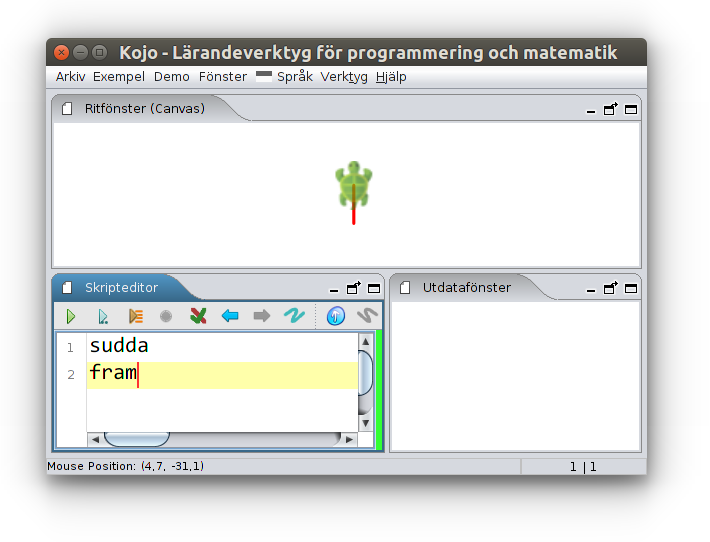
\includegraphics[width=0.7\textwidth]{../img/kojo}

\pause position, rikting, pennfärg, pennbredd, penna uppe/nere, fyllfärg
\end{Slide}



\begin{Slide}{Vad är ett objekt?}
\begin{itemize}
\item Ett objekt är en abstraktion som...
\begin{itemize}
  \item kan innehålla \Emph{data} som objektet ''håller reda på'' och
  \item kan erbjuda \Emph{operationer} som \emph{gör} något eller ger ett \emph{värde}
\end{itemize}

\pause

\item Exempel: Sköldpaddan i Kojo 
\includegraphics[width=0.08\textwidth]{../img/turtle.png}
\begin{itemize}
  \item Vilken \Emph{data} sparas av sköldpaddan?
  \pause
  \item[] position, rikting, pennfärg, ...

  \item Vilka \Emph{operationer} kan man be sköldpaddan att utföra?

  \item[] fram, höger, vänster, ...
  \pause


\end{itemize}

\item Terminologi:
\begin{itemize}
  \item objektets data sparas i variabler som kallas \Alert{attribut}
  \item alla variabelvärden utgör tillsammans objektets \Alert{tillstånd}
  \item operationerna är funktioner i objektet och kallas \Alert{metoder}
  \item attribut, metoder (och annat i objektet) kallas \Alert{medlemmar}
\end{itemize}
\end{itemize}
\end{Slide}



\begin{Slide}{Deklarera, allokera, referera}
Olika saker man kan göra med objekt:
\begin{itemize}
  \item \Emph{deklarera}: att skriva kod som beskriver objekt; \\
  finns flera sätt: singelobjekt, klass, tupel, ...
  \item \Emph{allokera}: att skapa plats i minnet för objektet vid körtid
  \item \Emph{referera}: att använda objektet via ett namn;\\
  man kommer åt innehållet i ett objekt med \Alert{punktnotation}: \\
  \code{ref.medlem}
  \pause
  \item (\Emph{avallokera}): att frigöra minne för objekt som inte längre används;
  detta \Alert{sker automatiskt} i Scala och Java, men i många andra språk,
  t.ex. C++, får man själv hålla reda på avallokering,
  vilket är knepigt och det blir lätt svåra buggar.
\end{itemize}
\end{Slide}


\begin{Slide}{Allokera objekt}\SlideFontSmall
Det finns flera olika sätt att skapa objekt:
\begin{itemize}

\item Använda en \Emph{färdig funktion} som skapar ett objekt åt oss:
\begin{Code}
Vector(1,2,3)   // skapar ett Vector-objekt
\end{Code}
{\SlideFontSmall En funktion som skapar objekt kallas \Alert{fabriksmetod}.\vspace{0.5em}}

\item Använda \code{new} (mer om detta senare: då behövs en klass):
\begin{Code}
new SimpleWindow(600, 400, "fönstertitel")  // skapar ett fönsterobjekt
\end{Code}
{\SlideFontSmall Med \code{new} kan man skapa \Alert{många upplagor} av samma typ av objekt.\vspace{0.5em}}

\item Deklarera ett \Emph{singelobjekt} med nyckelordet \code{object}
\begin{itemize}\SlideFontSmall
  \item Ett singelobjekt finns i exakt \Alert{en} upplaga.
  \item Det allokeras \Alert{automatisk} första gången man refererar objektet; \\
  man behöver inte, och kan inte, skriva \code{new}.
  \pause
  \item Medlemmar i ett Scala-singelobjekt motsvarar \jcode{static}-medlemmar i en Java/C++/C\#-klass.
\end{itemize}
\item Använda en \Emph{tupel}, exempel: \code{val p = (200, 300)}
\end{itemize}
\end{Slide}

\Subsection{Singelobjekt}

\begin{Slide}{Vad är ett singelobjekt?}
\begin{itemize}
\item Ett singelobjekt \Eng{singelton} deklareras med nyckelordet \code{object} och kan användas för att samla \Emph{medlemmar} \Eng{members} som \Alert{hör ihop}.
\item Kallas också \Emph{modul}.
\item Medlemmarna kan t.ex. vara \Emph{variabler} (\code{val}, \code{var}) och \Emph{metoder} (\code{def}). En \Alert{metod} är en \Emph{funktion} i ett objekt.
\item Exempel: singelobjekt/modul som hanterar highscore:
\begin{Code}
object Highscore {
  var highscore = 0
  def isHighscore(points: Int): Boolean = points > highscore
}
\end{Code}
\end{itemize}
\pause
{\SlideFontSmall Tanken är ofta att abstraktionen ska vara användbar i annan kod, för att underlätta när man bygger applikationer, och kallas då även ett API (Application Programming Interface). Exempel: ett highscore-API}
\end{Slide}


\begin{Slide}{Allokering: minne reserveras med plats för data}
\begin{Code}
object Highscore {
  var highscore = 0
  def isHighscore(points: Int): Boolean = points > highscore
}
\end{Code}
\pause
\begin{tikzpicture}[font=\large\sffamily]
\matrix [matrix of nodes, row sep=0, column 2/.style={nodes={rectangle,draw,minimum width=0.8cm}}] (mat)
{
\texttt{HighScore}   &  \makebox(10,10){ }\\
%\texttt{g2}   &  \makebox(16,12){ }\\
};
\node[cloud, cloud puffs=13.0, cloud ignores aspect, minimum width=2cm, minimum height=3.8cm,
 align=center, draw] (x) at (5.8cm, -1.5cm) {
 \begin{tabular}{r l}
 \texttt{highscore} & \fbox{~~~~~0~~} \\

 \end{tabular}
 };
\filldraw[black] (1.2cm,0.0cm) circle (3pt) node[] (ref) {};
 \draw [arrow, line width=0.7mm] (ref) -- (x);
% \node[cloud, cloud puffs=15.7, cloud ignores aspect, %minimum width=5cm, minimum height=2cm,
% align=center, draw] (g2) at (5cm, -2cm) {Gurka-\\objekt};
% \filldraw[black] (0.4cm,-0.4cm) circle (3pt) node[] (g2ref) {};
% \draw [arrow] (g2ref) -- (g2);
\end{tikzpicture}
\end{Slide}


\begin{Slide}{Punktnotation, tillståndsförändring med tilldelning}
\begin{REPLnonum}
scala> Highscore.isHighscore(5)
res0: Boolean = true

scala> Highscore.highscore = 42
\end{REPLnonum}
\pause
\begin{tikzpicture}[font=\large\sffamily]
\matrix [matrix of nodes, row sep=0, column 2/.style={nodes={rectangle,draw,minimum width=0.8cm}}] (mat)
{
\texttt{HighScore}   &  \makebox(10,10){ }\\
%\texttt{g2}   &  \makebox(16,12){ }\\
};
\node[cloud, cloud puffs=13.0, cloud ignores aspect, minimum width=2cm, minimum height=3.8cm,
 align=center, draw] (x) at (5.8cm, -1.5cm) {
 \begin{tabular}{r l}
 \texttt{highscore} & \fbox{~~~~42~~} \\

 \end{tabular}
 };
\filldraw[black] (1.2cm,0.0cm) circle (3pt) node[] (ref) {};
 \draw [arrow, line width=0.7mm] (ref) -- (x);
% \node[cloud, cloud puffs=15.7, cloud ignores aspect, %minimum width=5cm, minimum height=2cm,
% align=center, draw] (g2) at (5cm, -2cm) {Gurka-\\objekt};
% \filldraw[black] (0.4cm,-0.4cm) circle (3pt) node[] (g2ref) {};
% \draw [arrow] (g2ref) -- (g2);
\end{tikzpicture}
\end{Slide}


\begin{Slide}{Punktnotation och operatornotation}
Punktnotation på formen\\~\\
\code{objekt.metod(argument)}
\\~\\kan även skrivas med \Emph{operatornotation}:\\~\\
\code{objekt metod argument}
\\~\\Exempel:\\
\code{1 + 2}\\
\code{Highscore isHigscore 1000}

\end{Slide}


\begin{Slide}{Namnrymd och skuggning}
\begin{itemize}\SlideFontSmall
  \item En \Emph{namnrymd}\footnote{\url{https://sv.wikipedia.org/wiki/Namnrymd}}  \Eng{name space} är en omgivning (kontext) i vilken alla namn är unika. Genom att skapa flera olika namnrymder
  kan man undvika ''\Alert{krockar}'' mellan lika namn med olika betydelser (homonymer). \\
  Exempel: mejladresser \code{kim@företag1.se}  ~$\neq$~  \code{kim@företag2.se}
  \item Medlemmarna i ett singelobjekt finns i en egen namnrymd,
  där alla namn måste vara unika. De ''krockar'' inte med namn ''utanför'' objektet. Dock kan det förekomma \Alert{skuggning} \Eng{shadowing}:
\end{itemize}
\begin{Code}
object Game {

  val highscore = 42   // ett annat värde än Game.Highscore.highscore

  object Highscore {
    var highscore = 0  // ett annat värde än Game.highscore
    def isHighscore(points: Int): Boolean = points > highscore
  }
}
\end{Code}

\end{Slide}



\begin{Slide}{Inkapsling: att dölja interna delar}\SlideFontSmall
Med nyckelordet \code{private} döljs interna delar för omvärlden.
Privata medlemmar kan bara refereras \emph{innifrån} objektet.
Denna princip kallas \Emph{inkapsling} \Eng{encapsulation}.
\begin{CodeSmall}
object Highscore {
  private var myHighscore = 0        // namnet myHighscore syns ej utåt
  def highscore: Int = myHighscore   // en s.k. getter ger ett attributvärde
  def isHighscore(points: Int): Boolean = points > myHighscore
  def update(points: Int): Unit = if (isHighscore(points)) myHighscore = points
}
\end{CodeSmall}
\pause
Varför har man nytta av detta?
\begin{itemize}
  \item Förhindra att man av misstag ändrar objekts tillstånd på fel sätt.
  \item Förhindra användning av kod som i framtiden kan komma att ändras.
  \item Erbjuder en enklare ''utsida'' genom dölja komplexitet ''på insidan''.
  \item Inte ''skräpa ner'' namnrymden med ''onödiga'' namn.
\end{itemize}
Nackdelar:
\begin{itemize}
  \item Begränsar användningen, har ej tillgång till alla delar.
  \item Svårare att experimentera med ett API medan man försöker förstå det.
\end{itemize}
\end{Slide}



\begin{Slide}{Idiom: Privata variabler med understreck vid ''krock''}\SlideFontSmall
\Emph{Idiom}: (d.v.s ett typiskt, allmänt accepterat sätt att skriva kod)
\begin{itemize}
  \item Om namnet på en privat variabel krockar med namnet på en getter
  brukar man börja det privata namnet med ett understreck:
\end{itemize}

\begin{CodeSmall}
object Highscore {
  private var _highscore = 0
  def highscore: Int = _highscore
  def isHighscore(points: Int): Boolean = points > _highscore
  def update(points: Int): Unit = if (isHighscore(points)) _highscore = points
}
\end{CodeSmall}

\pause

(Detta problem uppkommer inte i Java m.fl. språk, där metoder och attribut finns i \emph{olika} namnrymder.
Men i Scala har man valt att principen om \Emph{enhetlig access} ska gälla; alla medlemmar finns därmed i en gemensam namnrymd.)

\end{Slide}


\begin{Slide}{Modul}

\begin{itemize}
  \item En modul samlar kod som utgör en sammanhållen, avgränsad \Emph{uppsättning abstraktioner} som kan användas av annan kod  för att lösa ett specifikt (del)problem.
  \item I Scala finns två sätt att skapa moduler:\footnote{\href{https://en.wikipedia.org/wiki/Modular_programming}{en.wikipedia.org/wiki/Modular\_programming}}
  \begin{itemize}
    \item \Emph{singelobjekt} med nyckelordet \code{object} och
    \item \Emph{paket} med nyckelordet \code{package}
    \pause
    \item Liknar varandra; t.ex. kan man använda punktnotation och göra \code{import} på medlemmar i både singelobjekt och paket.
    \pause
    \item Skillnader:
    \begin{itemize}
      \item paket medför att \Alert{underkataloger} för maskinkoden skapas vid kompilering
      \item paket innehåller inte variabler på topp-nivå; dessa behöver ligga inuti singelobjekt eller klasser
    \end{itemize}
    \item (I Scala kan man kombinera begreppen: \code{package object})
  \end{itemize}

\end{itemize}
\end{Slide}





\begin{Slide}{Exempel: singelobjektet med tillstånd} \SlideFontSmall
\begin{Code}[basicstyle=\ttfamily\fontsize{9}{11}\selectfont]
object mittBankkonto {
  val kontonr: Long        = 1234567L
  var saldo: Int           = 1000
  def ärSkuldsatt: Boolean = saldo < 0
}
\end{Code}
\begin{REPLnonum}
scala> mittBankkonto.saldo -= 25000

scala> mittBankkonto.ärSkuldsatt
res0: Boolean = true
\end{REPLnonum}

(Vi ska i nästa vecka se hur man med s.k. klasser kan skapa många upplagor av samma  typ av objekt, så att vi kan ha flera olika bankkonto.)
\end{Slide}



\begin{Slide}{Exempel: tillstånd, attribut}
Ett objekts \Emph{tillstånd} är den samlade uppsättningen av värden av alla de attribut som finns i objektet.
\begin{Code}[basicstyle=\ttfamily\fontsize{9}{11}\selectfont]
object mittBankkonto {
  val kontonr: Long        = 1234567L
  var saldo: Int           = 1000
  def ärSkuldsatt: Boolean = saldo < 0
}
\end{Code}
\begin{tikzpicture}[font=\large\sffamily]
\matrix [matrix of nodes, row sep=0, column 2/.style={nodes={rectangle,draw,minimum width=0.8cm}}] (mat)
{
\texttt{mittBankkonto}   &  \makebox(10,10){ }\\
%\texttt{g2}   &  \makebox(16,12){ }\\
};
\node[cloud, cloud puffs=13.0, cloud ignores aspect, minimum width=2cm, minimum height=3.8cm,
 align=center, draw] (x) at (5.8cm, -1.5cm) {
 \begin{tabular}{r l}
 \texttt{kontonr} & \fbox{1234567L} \\
 \texttt{saldo} & \fbox{1000}\\
 \end{tabular}
 };
\filldraw[black] (1.7cm,0.0cm) circle (3pt) node[] (ref) {};
 \draw [arrow, line width=0.7mm] (ref) -- (x);
% \node[cloud, cloud puffs=15.7, cloud ignores aspect, %minimum width=5cm, minimum height=2cm,
% align=center, draw] (g2) at (5cm, -2cm) {Gurka-\\objekt};
% \filldraw[black] (0.4cm,-0.4cm) circle (3pt) node[] (g2ref) {};
% \draw [arrow] (g2ref) -- (g2);
\end{tikzpicture}
\end{Slide}


\begin{Slide}{Tillståndsändring}

När en variabel tilldelas ett nytt värde sker en \Emph{tillståndsändring}. Ett \Emph{förändringsbart objekt} \Eng{mutable object} har ett \Emph{förändringsbart tillstånd} \Eng{mutable state}.

\begin{REPLnonum}
scala> mittBankkonto.saldo -= 25000

scala> mittBankkonto.saldo
res1: Int = -24000
\end{REPLnonum}
\begin{tikzpicture}[font=\large\sffamily]
\matrix [matrix of nodes, row sep=0, column 2/.style={nodes={rectangle,draw,minimum width=0.8cm}}] (mat)
{
\texttt{mittBankkonto}   &  \makebox(10,10){ }\\
%\texttt{g2}   &  \makebox(16,12){ }\\
};
\node[cloud, cloud puffs=13.0, cloud ignores aspect, minimum width=2cm, minimum height=3.8cm,
 align=center, draw] (x) at (5.8cm, -1.5cm) {
 \begin{tabular}{r l}
 \texttt{kontonr} & \fbox{1234567L} \\
 \texttt{saldo} & \fbox{-24000}\\
 \end{tabular}
 };
\filldraw[black] (1.7cm,0.0cm) circle (3pt) node[] (ref) {};
 \draw [arrow, line width=0.7mm] (ref) -- (x);
% \node[cloud, cloud puffs=15.7, cloud ignores aspect, %minimum width=5cm, minimum height=2cm,
% align=center, draw] (g2) at (5cm, -2cm) {Gurka-\\objekt};
% \filldraw[black] (0.4cm,-0.4cm) circle (3pt) node[] (g2ref) {};
% \draw [arrow] (g2ref) -- (g2);
\end{tikzpicture}
\end{Slide}

\Subsection{Paket}


\begin{Slide}{Deklarera paket}
Med nyckelordet \code{package} först i en kodfil ges alla deklarationer en gemensam namnrymd.\\
\vspace{1em}
Denna kod ligger i filen f1.scala:
\begin{Code}
package mittpaket

object A {
  def main(args: Array[String]) : Unit = B.hej
}
\end{Code}

Denna kod ligger i filen f2.scala:
\begin{Code}
package mittpaket

object B {
  def hej = println("hej mittpaket")
}
\end{Code}
Singelobjekten \code{A} och \code{B} finns båda i namnrymden \code{mittpaket}.
\end{Slide}

\begin{Slide}{Kompilera paket}\SlideFontSmall
Paketdeklarationer medför att kompilatorn placerar bytekodfiler i en katalog med samma namn som paketet:
\begin{REPL}
> scalac f1.scala f2.scala     // samkompilering av två filer
> ls
f1.scala  f2.scala  mittpaket
> ls mittpaket
A.class  A$.class  B.class  B$.class
> scala mittpaket.A
hej mittpaket
\end{REPL}
\pause
Idiom, syntax och semantik:
\begin{itemize}
  \item Paketnamn brukar bestå av enbart små bokstäver.
  \item Om paketnamn innehåller punkt(er), skapas nästlade underpaket, exempel:  \code{p1.p2.p3} kompilerar kod till katalogen \code{p1/p2/p3}
  \item Det är ovanligt, men man kan i Scala ha flera paket och även nästlade paket i \Alert{samma} kodfil
  om man använder klammerparenteser, exempel:
  \code|package p1 { object A; package p2 { object B }}|
\end{itemize}
\end{Slide}



\Subsection{Tupler}


\begin{Slide}{Vad är en tupel?}\SlideFontSmall

\begin{itemize}
\item En $n$-tupel är ett objekt som samlar $n$ st objekt i en enkel datastruktur med koncis syntax;
du behöver bara parenteser och kommatecken för att skapa tupel-objekt: ~~\code{(1,'a',"hej")}
\item Elementen kan alltså vara av \Alert{olika} typ.

\item
\code{(1,'a',"hej")} är en \Emph{3-tupel} av typen: \code{(Int, Char, String)}

\pause

\item Du kan komma åt de enskilda elementen med \Emph{\code{_1}}, \Emph{\code{_2}}, ...  \code{_}$n$

\begin{REPL}
scala> val t = ("hej", 42, math.Pi)
t: (String, Int, Double) = (hej,42,3.141592653589793)

scala> t._1
res0: String = hej

scala> t._2
res1: Int = 42
\end{REPL}

\pause

\item Tupler är praktiska när man inte vill ta det lite större arbetet att skapa en egen klass.
(Men med klasser kan man göra mycket mer än med tupler.)

\item I Scala kan du skapa tupler upp till en storlek av 22 element.
\\ (Behöver du fler element, använd i stället en samling, t.ex. \code{Vector}.)

\end{itemize}

\end{Slide}


\begin{Slide}{Tupler som parametrar och returvärde.}\SlideFontSmall

\begin{itemize}

\item Tupler är smidiga som \Emph{parametrar} om man vill kombinera värden som hör ihop, till exempel
 x- och y-värdena i en punkt: \code{(3, 4)}
\pause
\item Tupler är smidiga när man på ett enkelt och typsäkert sätt
vill låta en funktion \Emph{returnera mer än ett värde}.

\begin{REPL}
scala> def längd(p: (Double, Double)): Double = math.hypot(p._1, p._2)

scala> def vinkel(p: (Double, Double)): Double = math.atan2(p._1, p._2)

scala> def polär(p: (Double, Double)) = (längd(p), vinkel(p))

scala> polär((3,4))
res2: (Double, Double) = (5.0,0.6435011087932844)

\end{REPL}
\vspace{0.5em}
\item Om typerna passar kan man skippa dubbla parenteser vid \Emph{ensamt tupel-argument}:
\begin{REPL}
scala> polär(3,4)
res3: (Double, Double) = (5.0,0.6435011087932844)
\end{REPL}
\item[] {\SlideFontTiny\href{https://sv.wikipedia.org/wiki/Pol\%C3\%A4ra_koordinater}{https://sv.wikipedia.org/wiki/Polära\_koordinater}}


\end{itemize}
\end{Slide}



\begin{Slide}{Ett smidigt sätt att skapa 2-tupler med metoden \texttt{->}}
Det finns en metod vid namn \code{->} som kan användas på objekt av \Alert{godtycklig} typ för att \Emph{skapa par}:

\vspace{0.8em}
\begin{REPL}
scala> ("Ålder", 42)
res0: (String, Int) = (Ålder,42)

scala> "Ålder".->(42)
res1: (String, Int) = (Ålder,42)

scala> "Ålder" -> 42
res2: (String, Int) = (Ålder,42)

scala> Vector("Ålder" -> 42, "Längd" -> 178, "Vikt" -> 65)
res3: scala.collection.immutable.Vector[(String, Int)] =
        Vector((Ålder,42), (Längd,178), (Vikt,65))


\end{REPL}
\end{Slide}




\Subsection{Fördröjd initialisering}

\begin{Slide}{Lata variabler och fördröjd initialisering}
Med nyckelordet \code{lazy} före \code{val} skapas en s.k. ''lat'' \Eng{lazy} variabel.
\begin{REPL}
scala> val striktVektor = Vector.fill(1000000)(math.random)
striktVektor: scala.collection.immutable.Vector[Double] =
 Vector(0.7583305221813246, 0.9016192590993339, 0.770022134260162, 0.15667718184929746, ...

scala> lazy val latVektor = Vector.fill(1000000)(math.random)
latVektor: scala.collection.immutable.Vector[Double] = <lazy>

scala> latVektor
res0: scala.collection.immutable.Vector[Double] =
  Vector(0.5391685014341797, 0.14759775960530275, 0.722606095900537, 0.9025572787055386, ...
\end{REPL}

En \code {lazy val} initialiseras \Alert{inte} vid deklarationen utan när den \Alert{refereras första gången}. Yttrycket som anges i deklarationen evalueras med s.k. \Emph{fördröjd evaluering} (även ''lat'' evaluering).
\end{Slide}

\begin{Slide}{Vad är egentligen skillnaden mellan \texttt{val}, \texttt{var}, \texttt{def} och \texttt{lazy val}?}
\begin{Code}[basicstyle=\ttfamily\fontsize{8}{11}\selectfont]
object slump {
  val förAlltidSammaReferens  = math.random
  var kanÄndrasMedTilldelning = math.random
  def evaluerasVidVarjeAnrop  = math.random
  lazy val fördröjdInit       = Vector.fill(1000000)(math.random)
}
\end{Code}
\vspace{1em}\pause
Lat evaluering är en viktig princip inom funktionsprogrammering som möjliggör effektiva, oföränderliga datastrukturer där element allokeras först när de behövs. \\
\href{https://en.wikipedia.org/wiki/Lazy_evaluation}{en.wikipedia.org/wiki/Lazy\_evaluation}
\end{Slide}



\begin{Slide}{Singelobjekt är lata}

\begin{itemize}
  \item Singelobjekt allokeras \Alert{inte} direkt vid deklaration; allokeringen sker först då objektet refereras första gången.

\pause

  \item Exempel:

\end{itemize}

\begin{Code}
object mittLataObjekt {
  println("jag är lat")
  val storArray = { println("skapar stor Array"); Array.fill(10000)(42) }
  lazy val ännuStörreArray = Array.fill(Int.MaxValue)(42)
}
\end{Code}

När sker utskrifterna?

När allokeras variablerna?

\end{Slide}



\Subsection{Funktioner är objekt}

\begin{Slide}{Programmeringsparadigm}
\href{https://en.wikipedia.org/wiki/Programming_paradigm}{en.wikipedia.org/wiki/Programming\_paradigm}:
\begin{itemize}
\item \Emph{Imperativ programmering}: programmet är uppbyggt av sekvenser av olika satser som läser och \Alert{ändrar} tillstånd
\item \Emph{Objektorienterad programmering}: en sorts imperativ programmering där programmet består av objekt som kapslar in tillstånd och erbjuder operationer som läser och \Alert{ändrar} tillstånd.
\item \Emph{Funktionsprogrammering}: programmet är uppbyggt av samverkande (äkta) funktioner som \Alert{undviker} föränderlig data och tillståndsändringar. Oföränderliga datastrukturer skapar effektiva program i kombination med lat evaluering och rekursion.
\end{itemize}
\end{Slide}


\begin{Slide}{Funktioner är äkta objekt i Scala}
Scala visar hur man kan \Alert{förena} \Eng{unify} \\ \Emph{objekt-orientering} och \Emph{funktionsprogrammering}: \\\vspace{0.5em}

\textbf{En funktion är ett objekt som har en \code{apply}-metod.}
\pause
\begin{REPLnonum}
scala> object öka {
         def apply(x: Int) = x + 1
       }

scala> öka.apply(1)
res0: Int = 2

scala> öka(1)   // metoden apply behöver ej skrivas explicit
res1: Int = 2
\end{REPLnonum}
\end{Slide}



\begin{Slide}{Fördjupning: Äkta funktionsobjekt är av funktionstyp}
Egentligen, mer precist:\\
\textbf{En funktion är ett objekt \Alert{av funktionstyp} som har en \code{apply}-metod.}
\pause
\begin{REPLnonum}
scala> object öka extends (Int => Int) {
         def apply(x: Int) = x + 1
       }

scala> öka(1)
res2: Int = 2

scala> Vector(1,2,3).map(öka)
res3: scala.collection.immutable.Vector[Int] = Vector(2, 3, 4)

scala> öka.   // tryck TAB
andThen   apply   compose   toString
\end{REPLnonum}
Mer om \code{extends} senare i kursen... %extends (Int => Int skrivs om till Function1[Int, Int]
\end{Slide}



\Subsection{Använda färdiga klasser}

\begin{Slide}{Vad är en klass?}
En klass kan användas för att skapa många objekt av samma typ. Varje upplaga har sitt eget tillstånd och kallas en \Emph{instans} av klassen (mer om detta nästa vecka).
\begin{Code}
class BankKonto(val kontonr: Long, var saldo: Int)  {  // deklarera en klass
  def ärSkuldsatt: Boolean = saldo < 0
}
\end{Code}
\pause
\begin{REPL}
scala> val bk1 = new BankKonto(1234567L, 1000 )   // instansiera en klass
bk1: BankKonto = BankKonto@5d7399f9

scala> val bk2 = new BankKonto(6789012L, -200 )
bk2: BankKonto = BankKonto@286855ea

scala> bk1.saldo
res0: Int = 1000

scala> bk2.ärSkuldsatt
res1: Boolean = true
\end{REPL}
\end{Slide}

\begin{Slide}{Använda klassen \code{Color}}\SlideFontSmall
\begin{itemize}
\item I JDK8 (Java Development Kit version 1.8) finns 217 paket (moduler) och 4240 färdiga klasser.
\footnote{\SlideFontTiny\url{https://stackoverflow.com/questions/3112882/}}

\item En av dessa klasser heter \code{Color} och ligger i paketet \code{java.awt} och används för att representera RGB-färger med ett tal som beskriver andelen Rött, Grönt och Blått.
\end{itemize}
\begin{REPL}
scala> val röd = new java.awt.Color(255, 0, 0)    //  en maximalt röd färg

scala> import java.awt.Color  // namnet Color tillgängligt i aktuell namnrymd

scala> Color.    // tryck TAB och se alla publika medlemmar
\end{REPL}
\pause
\begin{itemize}
\item Använd klassen \code{java.awt.Color} på veckans övning.
\item Hur ska jag veta hur jag kan använda en färdig klass?
\pause
\begin{enumerate}\SlideFontTiny
  \item Läs koden, visar ''insidan'' med all sin komplexitet; kan vara knepigt...
  \item Läs \Emph{dokumentationen}, visar ''utsidan'' som är enklare (?) än ''insidan''
  \item \Alert{Experimentera} med hjälp av REPL och/eller en IDE
\end{enumerate}
\end{itemize}

\end{Slide}

\begin{Slide}{Skapa dokumentation}
\code{scaladoc} är ett program som tar Scala-kod som indata och skapar en webbsajt med dokumentation.

\vspace{2em}
\begin{tikzpicture}[node distance=1.5cm,scale=0.8, every node/.style={transform shape}]
\node (input) [startstop] {\texttt{src/*.scala}};

\node(inptext) [right of=input, text width=4cm, scale=1.2,xshift=4.5cm]{en katalog \texttt{src} som innehåller \texttt{.scala}-filer};

\node (scaladoc) [process, below of=input]
{\texttt{scaladoc}};

\node (output) [startstop, below of=scaladoc] {\texttt{index.html} ~~~med mera...};

\node(outtext) [right of=output, text width=4cm, scale=1.2,xshift=4.5cm]{En webbsajt};


\draw [arrow] (input) -- (scaladoc);
\draw [arrow] (scaladoc) -- (output);
\end{tikzpicture}

\vspace{2em} För Java-kod finns motsvarande program som heter \code{javadoc}.
\end{Slide}

\begin{Slide}{Använda dokumentation för färdiga klasser.}
\begin{itemize}
  \item Dokumentation för standardbiblioteket i Scala finns här:  \\ \url{https://www.scala-lang.org/api/}
  \item Övning: Leta upp dokumentationen för metoden \code{reduceLeft} i klassen \code{Vector}.
  \item[]
  \item Dokumentation för standardbiblioteket i Java finns här:  \\ \url{https://docs.oracle.com/javase/8/docs/api/}
  \item Övning: Leta upp dokumentationen för \code{java.awt.Color}

\end{itemize}
\end{Slide}


\begin{Slide}{Vad är en jar-fil?}
\begin{itemize}
  \item Förkortningen \Emph{jar} kommer från ''Java Archive''
  \item En \Emph{jar}-fil följer ett standardiserat filformat och används för att \Alert{paketera flera filer} i en och samma fil, exempelvis:
  \begin{itemize}
    \item \texttt{.class}-filer med bytekod
    \item resursfiler för en applikation t.ex. bilder \code{.png}, \code{.jpg}, etc
    \item information om vilken klass som innehåller \code{main}-funktionen
    \item etc.
  \end{itemize}
  \item En \code{.jar}-fil komprimeras på samma sätt som en \code{.zip}-fil.
  \item Fördjupning för den intresserade:\\
  {\SlideFontTiny\url{https://en.wikipedia.org/wiki/JAR_(file_format)}}
\end{itemize}
\end{Slide}


\begin{Slide}{Vad är \emph{classpath}?}\SlideFontSmall
\begin{itemize}
  \item Hur hittar kompilatorn färdiga moduler?
\pause
\item Kompilatorerna \code{scalac} och \code{javac} och programmen \code{scala} och \code{java} som kör igång JVM använder \Alert{en lista med filsökvägar} kallad \Emph{classpath} när de söker efter färdiga moduler.
\pause
\item Aktuellt bibliotek samt standardbiblioteket ligger per default på classpath.
\item Med hjälp av optionen \code{-classpath} eller kortare \code{-cp} kan annan classpath anges.
\item En lista med bibliotek separeras med kolon.\\(Windows: semikolon)
\item Det går bra att lägga jar-filer till listan med filsökvägar classpath.
\item Exempel: (punkt används för att ange aktuellt bibliotek)
\begin{REPLnonum}
scala -cp "lib/cslib.jar:." Main
\end{REPLnonum}
\end{itemize}
\end{Slide}


\begin{Slide}{Färdiga, enkla funktioner för att rita finns i klassen \texttt{cslib.window.SimpleWindow}}
På labben ska du använda \code{cslib.window.SimpleWindow}
\begin{itemize}
\item Jarfilen \code{cslib.jar} innehåller paketet \code{cslib} som innehåller paketet \code{window} som innehåller Java-klassen \code{SimpleWindow}.
%\item En \Emph{klass} är en ''mall'' för att göra \Emph{objekt}.
\item Med \code{SimpleWindow} kan man skapa ritfönster.
%\item När man skapar ett objekt från en klass använder man nyckelordet \code{new}.
\item Ladda ner \url{http://cs.lth.se/pgk/cslib} och lägg sedan jar-filen den katalog där du startar REPL med: \code{scala -cp cslib.jar}
\end{itemize}
\pause
\begin{REPLnonum}
> scala -cp cslib.jar
scala> val w = new SimpleWindow(200,200,"hejsan")
\end{REPLnonum}
\pause Studera dokumentationen för \code{cslib.window.SimpleWindow} här: \url{http://cs.lth.se/pgk/api/}
\end{Slide}




\ifkompendium\else


\Subsection{Veckans övning och laboration}

\begin{Slide}{Övning \texttt{objects}}\SlideFontTiny
\setlength{\leftmargini}{0pt}
\begin{itemize}
%!TEX encoding = UTF-8 Unicode
%!TEX root = ../exercises.tex

\item Kunna skapa och använda objekt som moduler.
%\item Kunna förklara vad ett block och en lokal variabel är.
%\item Kunna skapa och använda lokala funktioner och förklara nyttan med dessa.
\item Kunna förklara hur nästlade block påverkar namnsynlighet och namnöverskuggning.
\item Kunna förklara begreppen synlighet, privat medlem, namnrymd och namnskuggning.
%https://it-ord.idg.se/ord/overskuggning/

\item Kunna skapa och använda tupler.
\item Kunna skapa funktioner som har multipla returvärden.
\item Kunna förklara den semantiska relationen mellan funktioner och objekt i Scala.

\item Kunna förklara kopplingen mellan paketstruktur och kodfilstruktur.
\item Kunna använda en jar-fil och classpath.

\item Kunna använda import av medlemmar i objekt och paket.
\item Kunna byta namn vid import.

\item Kunna skapa och använda variabler med fördröjd initialisering.
\item Kunna förklara när parenteserna kan skippas runt tupel-argument.

\end{itemize}
\end{Slide}

\begin{Slide}{Lab \texttt{blockmole}}%\SlideFontTiny
%\setlength{\leftmargini}{0pt}
\begin{itemize}
\input{../compendium/modules/w04-objects-lab-goals.tex}
\end{itemize}

\end{Slide}
\fi


\Lecture{5}{Klasser}
\input{body/lect-w05-classes.tex}
\input{body/lect-w05-equality.tex}
\input{body/lect-w05-case-classes.tex}
\input{body/lect-w05-specifications.tex}
\input{body/lect-w05-muddiest-point.tex}
\input{body/lect-w05-assignments.tex}


\Lecture{6}{Sekvensalgoritmer}
\input{body/lect-w06-seq-insert-remove-copy.tex}
\input{body/lect-w06-varargs.tex}
\input{body/lect-w06-seq-append-insert-remove.tex}
\input{body/lect-w06-stringbuilder.tex}
\input{body/lect-w06-seq-choice.tex}
\input{body/lect-w06-scanner.tex}
\input{body/lect-w06-random.tex}
\input{body/lect-w06-register.tex}
\input{body/lect-w06-assignments.tex}

\Lecture{7}{Datastrukturer}
\input{body/lect-w07-datastruct.tex}
\input{body/lect-w07-tuples.tex}
\input{body/lect-w07-classes.tex}
\input{body/lect-w07-collections.tex}
\input{body/lect-w07-ide.tex}

\Lecture{8}{Matriser, typparametrar}
%!TEX encoding = UTF-8 Unicode
%!TEX root = ../lect-week08.tex

%%%

\ifkompendium\else

\Subsection{Kontrollskrivning}
\begin{Slide}{Resultat på kontrollskrivning 2016}
\pgfplotstableread[row sep=\\,col sep=&]{
    poäng & kamraträttat & korrigerat\\
    0     & 18  & 15\\
    1     & 29  & 29 \\
    2     & 17  & 15\\
    3     & 20  & 21 \\
    4     & 21  & 18 \\
    5     & 8   & 15 \\
    }\mydata

\begin{minipage}{0.6\textwidth}
\hspace*{-0.65cm}\begin{tikzpicture}[scale=0.9, every node/.style={scale=0.9}]
    \begin{axis}[
            ybar,
            symbolic x coords={0,1,2,3,4,5},
            xtick=data,
            nodes near coords,
            nodes near coords align={vertical},
            legend style={at={(0.5,1)},anchor=south,legend columns=-1,draw=none},
            ymin=0,ymax=35,
            ylabel={Antal},
            xlabel={Poäng},
        ]
        \addplot table[x=poäng,y=kamraträttat]{\mydata};
        \addplot table[x=poäng,y=korrigerat]{\mydata};
        \legend{kamraträttat, korrigerat}
    \end{axis}
\end{tikzpicture}
\end{minipage}%
\begin{minipage}{0.35\textwidth}
\begin{itemize}\SlideFontTiny
\item[] Totalt: 107 st (100\%)
\item[] 4 -- 5: 33st (29\%)
\item[] 3 -- 5: 54st (48\%)
\item[] 0 -- 2: 59st (52\%)
\item[] 0 -- 1: 44st (39\%)
\end{itemize}
\end{minipage}%


\end{Slide}

\begin{Slide}{Genomgång av kontrollskrivning}
\begin{itemize}
\item Förstå uppgiften

\item Strategi för lösning

\item Skapa lösning iterativt

\item Kontrollera lösning
\end{itemize}
\end{Slide}



\Subsection{REBOOT CAMP}

\begin{Slide}{REBOOT CAMP}
\Large

Träffas i samarbetsgrupper och organisera en \Alert{reboot-camp} baserat på kontrollskrivningsresultatet.

~\\

3-5: GRATTIS! Bli ännu starkare!

0-2: Fixa trösklar och luckor!

\vspace{0.5em} \Emph{STAY CALM} \\\vspace{0.5em} \Alert{GET ON TRACK}
\end{Slide}

%
% \begin{Slide}{Omplanering: w08 = REBOOT CAMP}\SlideFontSmall
% Det är \Alert{för många} som ligger \Alert{för långt efter}: \\
% \Emph{Vi måste göra något!}
% \begin{itemize}
% \item Omplanering: w08 = REBOOT CAMP
% \begin{itemize}\SlideFontTiny
% \item \Alert{GE JÄRNET} för att stärka dig inför resten av kursen!
% \item Noggrann genomgång av kontrollskrivning
% \item Gör självdiagnostik och kämpa dig över trösklar och fyll igen luckor
% \item Slipa dina inlärningsverktyg!
% \item Resurstider: \code{reboot-init}: \Emph{planera, arbeta}
% \item Labb: \code{reboot-check}: \Emph{visa hur det går, arbeta}
% \end{itemize}
% \item Vi senarelägger alla kvarvarande labbar en vecka så att w08 frigörs;
%  lab \code{chords-team} görs alltså i vecka w09 etc.
%
% \item Sista labben \code{life} omdefinieras till att ingå bland projektalternativen i slutet av kursen (man får ändå öva på matriser på lab \code{maze})
%
% \item Stoffet i veckorna w12 \& w13 slås ihop och minskas ned
%
% \item Övn threads blir frivilligt extramaterial och ingår ej i examinationen.
%
% \end{itemize}
% \end{Slide}


%\Subsection{Slipa verktygen}

\begin{Slide}{Slipa verktygen}
För dig som har det \Alert{svårt}:
\begin{itemize}
\item Man kan inte lära sig ett språk bara genom att \Alert{passivt} läsa
\item Om du inte börjat än: nu måste du verkligen börja skriva, prata, uppfinna, konstruera, göra själv, vara \Emph{aktiv}, ...
\end{itemize}
För dig som har det \Emph{lätt}:
\begin{itemize}
\item Om du utmanar dig når du \Emph{mycket} längre
\item Analysera dina styrkor och svagheter
\item Utveckla din studieteknik och problemlösningsförmåga
\end{itemize}
\end{Slide}

\begin{Slide}{Vad avgör studieframgång?}
Studieteknik, Attityd till sina studier, (Talang)
\url{https://www.youtube.com/watch?v=gSbpRjxYq24}

\vspace{2em} Att repetera:
\url{https://www.youtube.com/watch?v=mmAmsaRH_VA}

\vspace{2em} Att planera:
\url{https://www.youtube.com/watch?v=g2BTFzYnNNY}
\end{Slide}

\begin{Slide}{Självdiagnostik och planering}
\begin{itemize}
\item Hur lär jag mig bäst?
\item Vad behöver jag extra träning på?
\begin{itemize}
\item Vad hade jag lätt resp. svårt för på kontrollskrivingen?
\item Vilka är mina \Alert{trösklar}? Extra svårt?
\item Vilka är mina \Alert{luckor}? Inte provat alls?
\item Vilka är mina \Emph{intressen}? Hur fördjupa mig?
\end{itemize}
\item Hur ska jag planera min REBOOT CAMP?
\begin{itemize}
\item Gör ett schema dag för dag.
\item Vilken undervisning ska jag gå på?
\item Du som fick 0-2: gå på minst 2 resurstider.
\item Hur mycket fritid kan jag frigöra till REBOOT CAMP?
\end{itemize}
\end{itemize}
\end{Slide}



\begin{Slide}{Strategier för problemlösning i programmering}
\begin{itemize}
\item Börja med ett litet men fungerande program; ta sedan många små steg och testa hela tiden att det fungerar
\item Om problemet är för \Alert{svårt}:\\ lös först ett \Emph{lättare}, relaterat problem
\item Dela upp problemet i delar
\begin{itemize}
\item \code{val braNamn = delresultat}
\item \code{def delLösning = algoritm som löser delproblem}
\item \code{??? // inte klart än}
\end{itemize}
\item Problemlösning är inte linjärt: du måste kunna knåpa på ditt program i olika ''ändar''; skriva lite här och där; stoppa in; flytta runt; ändra
\end{itemize}
\end{Slide}

\begin{Slide}{Strategier för att komma över trösklar}\SlideFontSmall
\Alert{tröskel} == jag har svårt att begripa och komma vidare; kan ej själv konstruera

\begin{itemize}\SlideFontTiny
\item Du måste först \Emph{identifiera tröskeln} och tydligt formulera vad du inte förstår eller inte kan klara av att själv skapa.

\item Du måste hitta ett sätt att \Emph{konkretisera} begrepp och \Emph{visualisera} vad som händer \\
Använd analogier: kaffekvarnen för funktion, stämpla för instansiering, etc.

\item Använd flera exempel på samma sak: försök se \Emph{mönster} \\
Exempel: Tomat och Gurka är Grönsak; Student och Lärare är Person. \\ Lär dig pseudokodexempel på vanliga algoritmer i kompendiet utantill!

\item Gör \Emph{enklast möjliga} exempel som du exekverar: \\ Skapa en enkel klass med bara en heltalsmedlem och ''lek'' med den.

\item Bygg vidare på det du lär dig och \Emph{utvidga} stegvis med större exempel.\\ Exekvera allt större kod som du själv skriver!

\item \Emph{Avancera}: Kombinera med begrepp du redan känner. Exekvera!

\end{itemize}
Utgå från det du vet om hur just \Emph{du} lär dig bäst. Hur ska du vara \Alert{aktiv}? \\ Rita. Prata. Skriv sammanfattningar. Skapa egna program. ...
\end{Slide}

\begin{Slide}{Uppdrag under rasten}
\begin{itemize}
\item Tala med med en eller två som är \Emph{ungefär på din nivå} med ledning av resultatet på kontrollskrivningen. (Eller skriv ner för dig själv om du helst vill vara ensam)

\item 5 minuter var: berätta för den andre om...
\begin{itemize}
 \item dina trösklar: vad är extra svårt?
 \item dina luckor: vad har jag inte ens provat själv?
 \item dina fördjupningsintressen: vad vill jag veta mer om?
 \item övningar och laborationer som behöver kompletteras
\end{itemize}
\item \Alert{Fastna inte} i orsaker/ursäkter till situationen: \Emph{utgå från nuläget} och  indentifiera trösklar/luckor/fördjupning
\end{itemize}
\end{Slide}


\begin{Slide}{Tillbaka efter rasten:}
Påbörja detta arbete som du sedan fortsätter med i eftermiddag/kväll:
\begin{itemize}
\item Gör en lista på vad \Alert{du} behöver göra för att slipa dina \Alert{studieverktyg} i programmering?
\item För varje begreppslista i w01-w07:
\begin{itemize}
\item Välj ut några begrepp som är viktiga för dig att träna mer på.
\item Välj ut några övningar som är kopplade till begreppen.
\item Gör en prioriteringsordning för begreppen/övningarna.
\item Planera ditt arbete för veckan:
\begin{itemize}
\item Övningar
\item Ev. labbar att komplettera
\end{itemize}
\end{itemize}
\end{itemize}
Fortsätt detta jobb individuellt idag och\\
\Emph{ta med dig priolistan} till \\ \Alert{morgondagens föreläsning och till resurstiderna!}
\end{Slide}


%\Subsection{Prioritera dina uppgifter}

\begin{Slide}{Inventering av trösklar, luckor, fördjupning}
I ditt arbete med att identifiera trösklar, luckor, fördjupning kan du använda:
\begin{itemize}
\item Kontrollskrivningen
\item Målen på övningarna
\item Begreppslistan i varje modul
\end{itemize}
Gör en inventering och markera det du har någorlunda koll på och det du tycker är extra svårt (tröskel) eller sådant du missat (luckor). Om du är redo för fördjupning markera intressanta delar att lära dig mer om.
\end{Slide}

\begin{Slide}{Prioritera och definiera dina anpassade träning}
\begin{itemize}
\item Gör klart eventuella labbar som behöver kompletteras.
\item Välj en lagom stor mängd övningar ur kompendiet som hjälper dig med trösklar och luckor. Modifiera gärna övningarna efter dina behov.
\item Definiera ett program du ska jobba med fram till och med reboot-check.
\end{itemize}
\end{Slide}

% \begin{Slide}{Hur blir jag godkänd på reboot-check?}
% \begin{itemize}
% \item Förbered en kort genomgång som du ska göra när du får tid med handledare:
% \begin{itemize}
% \item Vilka trösklar/luckor/fördjupningar har du identifierat?
% \item Vad har du gjort under veckan?
% \item Visa ditt program som du jobbar med under labben och förklara hur programmet hänger ihop med dina trösklar/luckor/fördjupningar?
% \end{itemize}
% \item Använd tiden under labben till något vettigt;  jobba vidare på ditt eget program medan du väntar.
% \end{itemize}
% Du blir godkänd om du kan resonera om kopplingen mellan dina behov och dina åtgärder.
% \end{Slide}

\fi

%!TEX encoding = UTF-8 Unicode
%!TEX root = ../lect-w08.tex

%%%

\Subsection{Veckans labb: \texttt{maze}}
\begin{Slide}{Veckans labb: \texttt{maze}}\SlideFontSmall
Grunduppgift:
\begin{itemize}
\item Implementera en algoritm som hittar ut ur en labyrint.

\item En labyrint representeras av en \Emph{matris}, \\närmare bestämt en \Emph{vektor av vektorer} med  \Alert{booelska} värden: \\ \code{Vector[Vector[Boolean]]}

\pause Där de två olika sanningsvärdena representerar följande:
\begin{itemize}\SlideFontSmall
\item \code{true} om det \Emph{finns en vägg} på en viss plats i matrisen
\item \code{false} om det \Alert{inte} finns en vägg på en viss plats i matrisen

\end{itemize}
\pause
\item Använd enkel idé (som inte ger kortaste vägen): \\ Behåll vänster hand i kontakt med väggen och gå tills du når utgången.

\item Vad krävs av labyrinten för att detta ska fungera?
\end{itemize}
\pause Extrauppgift:
\begin{itemize}
\item Generera slumpmässig labyrint
\item Algoritmen (\emph{Prims algoritm}) är given i pseudokod
\end{itemize}

\end{Slide}

\begin{Slide}{Labyrint som booelsk matris}
\includegraphics[width=1.0\textwidth]{../img/w09-lab/MazeAndMatrix.jpg}
\end{Slide}

\begin{Slide}{Slumpmässig labyrint}
\includegraphics[width=0.68\textwidth]{../img/w09-lab/RandomMaze.jpg}
\end{Slide}

\Subsection{Matriser}

\begin{Slide}{Vad är en matris?}\SlideFontSmall
\begin{itemize}

\item En \Emph{matris} inom \Alert{matematiken} innehåller \Emph{rader} och \Emph{kolumner}\footnote{även kallade \emph{kolonner}} med tal.

\item I en \Alert{matematisk} matris har alla rader \Emph{lika många} element och

\item även alla kolumner har \Emph{lika många} element.

\item En matris av dimension $2\times{}5$ har $2 \cdot 5 = 10$ stycken element.

\item Exempel på en matematisk matris av dimension $2\times{}5$:
\[
M_{2,5}=
  \begin{pmatrix}
    5 & 2 & 42 & 4 & 5 \\
    3 & 4 & 18 & 6 & 7
  \end{pmatrix}
\]
\end{itemize}
\end{Slide}

\begin{Slide}{Indexering i en matris}\SlideFontSmall
\begin{itemize}

  \item En matris av dimension $m\times{}n$ har $m \cdot n$ stycken element.

  \item En matris $A_{m,n}$ av dimension $m\times{}n$ ritas inom matematiken ofta så här:

  \[
  A_{m,n} =
   \begin{pmatrix}
    a_{1,1} & a_{1,2} & \cdots & a_{1,n} \\
    a_{2,1} & a_{2,2} & \cdots & a_{2,n} \\
    \vdots  & \vdots  & \ddots & \vdots  \\
    a_{m,1} & a_{m,2} & \cdots & a_{m,n}
   \end{pmatrix}
  \]


\item Matrisindexering inom matematiken sker ofta från $1$, men ofta från $0$ i datorprogram.

\item Vad har talet $42$ för index i matrisen $M_{2,5}$ nedan?
\begin{itemize}\SlideFontTiny
  \item[--] Inom matematiken?
  \item[--] I Scala och Java och många andra språk?

  \[
  M_{2,5}=
    \begin{pmatrix}
      5 & 2 & 42 & 4 & 5 \\
      3 & 4 & 18 & 6 & 7
    \end{pmatrix}
  \]
\end{itemize}
\end{itemize}
\end{Slide}

\begin{Slide}{En matris med array av arrayer}
Inom programmering används ordet \Emph{matris} ofta för att beteckna en \Alert{nästlade struktur} i två dimensioner, till exempel en instans av typen \code{Array[Array[Int]]}
\begin{REPL}
scala> val xss = Array(Array(5,2,42,4,5),Array(3,4,18,6,7))
xss: Array[Array[Int]] = Array(Array(5, 2, 42, 4, 5), Array(3, 4, 18, 6, 7))
\end{REPL}
\pause
Man indexerar i en nästlad sekvens med upprepad \code{apply}:
\begin{REPL}
scala> xss(0)(2)
res0: ???                   // Vad är typ och värde?

scala> xss.apply(0).apply(2)
res1: ???                   // Vad är typ och värde?

scala> xss(0)
res2: ???                   // Vad är typ och värde?
\end{REPL}

\end{Slide}

\begin{Slide}{En matris med array av arrayer}
Inom programmering används ordet \Emph{matris} ofta för att beteckna en \Alert{nästlade struktur} i två dimensioner, till exempel en instans av typen \code{Array[Array[Int]]}
\begin{REPL}
scala> val xss = Array(Array(5,2,42,4,5),Array(3,4,18,6,7))
xss: Array[Array[Int]] = Array(Array(5, 2, 42, 4, 5), Array(3, 4, 18, 6, 7))
\end{REPL}

Man indexerar i en nästlad sekvens med upprepad \code{apply}:
\begin{REPL}
scala> xss(0)(2)
res0: Int = 42

scala> xss.apply(0).apply(2)
res1: Int = 42

scala> xss(0)
res2: Array[Int] = Array(5, 2, 42, 4, 5)
\end{REPL}
\end{Slide}

\begin{Slide}{Uppdatering av en förändringsbar nästlad struktur}
Man kan förändra en array av arrayer ''på plats'' med tilldelning:
\begin{REPL}
scala> val xss = Array(Array(5,2,42,4,5),Array(3,4,18,6,7))

scala> xss(0)(0) = 100

scala> xss
res0: ???

scala> xss(0)(2) = xss(0)(2) - 1

scala> xss
res1: ???

scala> xss(1) = Array.fill(5)(-1)

scala> xss
res2: ???
\end{REPL}
\end{Slide}

\begin{Slide}{Uppdatering av en förändringsbar nästlad struktur}
Man kan förändra en array av arrayer ''på plats'' med tilldelning:
\begin{REPL}
scala> val xss = Array(Array(5,2,42,4,5),Array(3,4,18,6,7))

scala> xss(0)(0) = 100

scala> xss
res0: Array[Array[Int]]=Array(Array(100, 2, 42, 4, 5), Array(3, 4, 18, 6, 7))

scala> xss(0)(2) = xss(0)(2) - 1

scala> xss
res1: Array[Array[Int]]=Array(Array(100, 2, 41, 4, 5), Array(3, 4, 18, 6, 7))

scala> xss(1) = Array.fill(5)(-1)

scala> xss
res2: Array[Array[Int]]=Array(Array(100, 2, 41, 4, 5), Array(-1,-1,-1,-1,-1))
\end{REPL}
\end{Slide}

\begin{Slide}{Några olika sätt att skapa förändringsbara matriser}\SlideFontSmall
Det jobbiga, primitiva sättet:
\begin{REPL}
scala> val xs = new Array[Array[Int]](2)
xs: Array[Array[Int]] = Array(null, null)

scala> for (i <- xs.indices) {xs(i) = new Array[Int](5)}

scala> xs
res0: Array[Array[Int]] = Array(Array(0, 0, 0, 0, 0), Array(0, 0, 0, 0, 0))

scala> println(xs)
[[I@196a99d0
\end{REPL}
Enklare sätt:
\begin{REPL}
scala> val xs = Array.ofDim[Int](2,5)
xs: Array[Array[Int]] = Array(Array(0, 0, 0, 0, 0), Array(0, 0, 0, 0, 0))
\end{REPL}
Enklare och tydligare sätt, där initialvärdet anges explicit:
\begin{REPL}
scala> Array.fill(2,5)(0)
res37: Array[Array[Int]] = Array(Array(0, 0, 0, 0, 0), Array(0, 0, 0, 0, 0))
\end{REPL}

\end{Slide}

\begin{Slide}{Exempel på skapande av oföränderlig nästlad struktur}\SlideFontSmall
Om du kan beräkna initialvärde direkt, använd \code{Vector.fill}:\\
{\SlideFontTiny\code{def fill[A](n1: Int, n2: Int)(elem: => A): Vector[Vector[A]]}}
\begin{REPL}
scala> Vector.fill(2,5)(scala.util.Random.nextInt(6) + 1)
res0:
  typ???
  värde???

\end{REPL}
Om du kan beräkna initialvärde ur index, använd \code{Vector.tabulate}:\\
{\SlideFontTiny\code{def tabulate[A](n1: Int, n2: Int)(f: (Int, Int) => A): Vector[Vector[A]]}}
\begin{REPL}
scala> Vector.tabulate(5,2)((x,y) => x + y + 1)
res1:
  typ???
  värde???

\end{REPL}
\end{Slide}

\begin{Slide}{Exempel på skapande av oföränderlig nästlad struktur}\SlideFontSmall
Om du kan beräkna initialvärde direkt, använd \code{Vector.fill}:\\
{\SlideFontTiny\code{def fill[A](n1: Int, n2: Int)(elem: => A): Vector[Vector[A]]}}
\begin{REPL}
scala> Vector.fill(2,5)(scala.util.Random.nextInt(6) + 1)
res0:
  scala.collection.immutable.Vector[scala.collection.immutable.Vector[Int]] =
  Vector(Vector(1, 2, 6, 2, 1), Vector(1, 4, 3, 3, 2))

\end{REPL}
Om du kan beräkna initialvärde ur index, använd \code{Vector.tabulate}:\\
{\SlideFontTiny\code{def tabulate[A](n1: Int, n2: Int)(f: (Int, Int) => A): Vector[Vector[A]]}}
\begin{REPL}
scala> Vector.tabulate(5,2)((x,y) => x + y + 1)
res1:
  scala.collection.immutable.Vector[scala.collection.immutable.Vector[Int]] =
  Vector(Vector(1,2), Vector(2,3), Vector(3,4), Vector(4,5), Vector(5,	6))

\end{REPL}
\end{Slide}



\begin{Slide}{Uppdatering av en oföränderlig nästlad struktur}\SlideFontSmall
Uppdatering av endimensionell struktur med \code{xs.updated}:\\
{\SlideFontTiny\code{def updated[A](index: Int, elem: A): Vector[A]} }
\begin{REPL}
scala> var xs = Vector.tabulate(5)(x => x + 1)
xs: typ??? = värde???

scala> xs = xs.updated(1, 42)
xs: typ??? = värde???
\end{REPL}

Uppdatering av nästlad struktur i två dimensioner:
\begin{REPL}
scala> var xss = Vector.tabulate(2, 5)((x,y) => x + y + 1)
xss:
  typ??? =
  värde???

scala> xss = xss.updated(0, xss(0).updated(1, 42))
xss:
  typ??? =
  värde???
\end{REPL}

\end{Slide}



\begin{Slide}{Uppdatering av en oföränderlig nästlad struktur}\SlideFontSmall
Uppdatering av endimensionell struktur med \code{xs.updated}:\\
{\SlideFontTiny\code{def updated[A](index: Int, elem: A): Vector[A]} }
\begin{REPL}
scala> var xs = Vector.tabulate(5)(x => x + 1)
xs: scala.collection.immutable.Vector[Int] = Vector(1, 2, 3, 4, 5)

scala> xs = xs.updated(1, 42)
xs: scala.collection.immutable.Vector[Int] = Vector(1, 42, 3, 4, 5)
\end{REPL}

Uppdatering av nästlad struktur i två dimensioner:
\begin{REPL}
scala> var xss = Vector.tabulate(2, 5)((x,y) => x + y + 1)
xss:
  scala.collection.immutable.Vector[scala.collection.immutable.Vector[Int]] =
  Vector(Vector(1, 2, 3, 4, 5), Vector(2, 3, 4, 5, 6))

scala> xss = xss.updated(0, xss(0).updated(1, 42))
xss:
  scala.collection.immutable.Vector[scala.collection.immutable.Vector[Int]] =
  Vector(Vector(1, 42, 3, 4, 5), Vector(2, 3, 4, 5, 6))
\end{REPL}

\end{Slide}


\begin{Slide}{Iterera över nästlad struktur: for-sats}\SlideFontSmall
Iterera med nästlad for-sats:
\begin{REPL}
scala> val xss = Vector.tabulate(2,5)((x,y) => x + y + 1)

scala> for (???) {
         for (???) {
           print(xss(i)(j) + " ")
         }
         println
       }

1 2 3 4 5
2 3 4 5 6
\end{REPL}
\end{Slide}

\begin{Slide}{Iterera över nästlad struktur: for-sats}\SlideFontSmall
Iterera med nästlad for-sats:
\begin{REPL}
scala> val xss = Vector.tabulate(2,5)((x,y) => x + y + 1)

scala> for (i <- xss.indices) {
         for (j <- xss(i).indices) {
           print(xss(i)(j) + " ")
         }
         println
       }

1 2 3 4 5
2 3 4 5 6
\end{REPL}
\end{Slide}


\begin{Slide}{Övningsexempel: Yatzy}\SlideFontSmall
Skapa en funktion \code{roll} som ger utfallet av n st tärningskast:
\begin{REPL}
scala> import scala.util.Random

scala> def roll(n: Int): Vector[Int] = ???
\end{REPL}

Skapa en funktion \code{isYatzy} som ger \code{true} om alla utfall är lika:
\begin{REPL}
scala> def isYatzy(xs: Vector[Int]): Boolean = ???
\end{REPL}
Du kan anta att xs.length > 0\\
Tips: använd metoden xs.forall: \\
\code{def forall[A](p: A => Boolean): Boolean }
\end{Slide}


\begin{Slide}{Övningsexempel: Yatzy}\SlideFontSmall
Skapa en funktion \code{roll} som ger utfallet av n st tärningskast:
\begin{REPL}
scala> import scala.util.Random

scala> def roll(n: Int): Vector[Int] = Vector.fill(n)(Random.nextInt(6) + 1)
\end{REPL}

Skapa en funktion \code{isYatzy} som ger \code{true} om alla utfall är lika:
\begin{REPL}
scala> def isYatzy(xs: Vector[Int]): Boolean = xs.forall(x => x == xs(0))
\end{REPL}
Du kan anta att xs.length > 0\\
Tips: använd metoden xs.forall: \\
\code{def forall[A](p: A => Boolean): Boolean }
\end{Slide}

\begin{Slide}{Iterera över nästlad struktur: for-sats}\SlideFontSmall
Iterera med nästlad for-sats: (vad har xss för typ?)
\begin{REPL}
scala> val xss = Vector.fill(100)(roll(5))

scala> for (???) {
         for (???) {
           print(s"($i)($j) == " + xss(i)(j) + " ")
         }
         println(isYatzy(???))
       }

(0)(0) == 5 (0)(1) == 3 (0)(2) == 4 (0)(3) == 1 (0)(4) == 3 false
(1)(0) == 3 (1)(1) == 3 (1)(2) == 6 (1)(3) == 3 (1)(4) == 1 false
(2)(0) == 3 (2)(1) == 4 (2)(2) == 2 (2)(3) == 2 (2)(4) == 1 false
(3)(0) == 5 (3)(1) == 2 (3)(2) == 6 (3)(3) == 5 (3)(4) == 1 false
(4)(0) == 4 (4)(1) == 6 (4)(2) == 4 (4)(3) == 1 (4)(4) == 4 false
(5)(0) == 3 (5)(1) == 4 (5)(2) == 6 (5)(3) == 5 (5)(4) == 1 false
(6)(0) == 4 (6)(1) == 6 (6)(2) == 2 (6)(3) == 2 (6)(4) == 6 false
(7)(0) == 2 (7)(1) == 5 (7)(2) == 3 (7)(3) == 6 (7)(4) == 2 false
(8)(0) == 4 (8)(1) == 4 (8)(2) == 6 (8)(3) == 1 (8)(4) == 4 false
(9)(0) == 3 (9)(1) == 3 (9)(2) == 3 (9)(3) == 3 (9)(4) == 3 true
(10)(0) == 1 (10)(1) == 2 (10)(2) == 4 (10)(3) == 3 (10)(4) == 3 false
(11)(0) == 6 (11)(1) == 5 (11)(2) == 4 (11)(3) == 1 (11)(4) == 5 false
(12)(0) == 3 (12)(1) == 6 (12)(2) == 6 (12)(3) == 4 (12)(4) == 2 false
\end{REPL}
\end{Slide}

\begin{Slide}{Iterera över nästlad struktur: for-sats}\SlideFontSmall
Iterera med nästlad for-sats: (xss är en \code{Vector[Vector[Int]]})
\begin{REPL}
scala> val xss = Vector.fill(100)(roll(5))

scala> for (i <- xss.indices) {
         for (j <- xss(i).indices) {
           print(s"($i)($j) == " + xss(i)(j) + " ")
         }
         println(isYatzy(xss(i)))
       }

(0)(0) == 5 (0)(1) == 3 (0)(2) == 4 (0)(3) == 1 (0)(4) == 3 false
(1)(0) == 3 (1)(1) == 3 (1)(2) == 6 (1)(3) == 3 (1)(4) == 1 false
(2)(0) == 3 (2)(1) == 4 (2)(2) == 2 (2)(3) == 2 (2)(4) == 1 false
(3)(0) == 5 (3)(1) == 2 (3)(2) == 6 (3)(3) == 5 (3)(4) == 1 false
(4)(0) == 4 (4)(1) == 6 (4)(2) == 4 (4)(3) == 1 (4)(4) == 4 false
(5)(0) == 3 (5)(1) == 4 (5)(2) == 6 (5)(3) == 5 (5)(4) == 1 false
(6)(0) == 4 (6)(1) == 6 (6)(2) == 2 (6)(3) == 2 (6)(4) == 6 false
(7)(0) == 2 (7)(1) == 5 (7)(2) == 3 (7)(3) == 6 (7)(4) == 2 false
(8)(0) == 4 (8)(1) == 4 (8)(2) == 6 (8)(3) == 1 (8)(4) == 4 false
(9)(0) == 3 (9)(1) == 3 (9)(2) == 3 (9)(3) == 3 (9)(4) == 3 true
(10)(0) == 1 (10)(1) == 2 (10)(2) == 4 (10)(3) == 3 (10)(4) == 3 false
(11)(0) == 6 (11)(1) == 5 (11)(2) == 4 (11)(3) == 1 (11)(4) == 5 false
(12)(0) == 3 (12)(1) == 6 (12)(2) == 6 (12)(3) == 4 (12)(4) == 2 false
\end{REPL}
\end{Slide}


\begin{Slide}{Iterera över nästlad struktur med nästlad foreach}\SlideFontSmall
Iterera med nästlad foreach-sats:
\begin{REPL}
scala> val xss = Vector.tabulate(2,5)((x,y) => x + y + 1)

xss.foreach{ xs => ??? ; println }

1 2 3 4 5
2 3 4 5 6
\end{REPL}
\end{Slide}


\begin{Slide}{Iterera över nästlad struktur med nästlad foreach}\SlideFontSmall
Iterera med nästlad foreach-sats:
\begin{REPL}
scala> val xss = Vector.tabulate(2,5)((x,y) => x + y + 1)

xss.foreach{ xs => xs.foreach{ x => print(x + " ") }; println }

1 2 3 4 5
2 3 4 5 6
\end{REPL}
\end{Slide}


\begin{Slide}{Nästlade for-uttryck}\SlideFontSmall
Iterera med \Emph{nästlad for-yield}:\\
%Statisk typ: \code{IndexedSeq[IndexedSeq[[Int]]} \\
%Dynamisk typ: \code{Vector[Vector[[Int]]}

\begin{REPL}
scala> val xss = for (i <- 1 to 2) yield {
                   for (j <- 1 to 5) yield i + j + 1
                 }
xss:
  scala.collection.immutable.IndexedSeq[
    scala.collection.immutable.IndexedSeq[Int]] =
      ???

\end{REPL}
Om man skriver så här får man en endimensionell struktur:
\begin{REPL}
scala> val xs = for (i <- 1 to 2; j <- 1 to 5) yield i + j + 1
xs:
  scala.collection.immutable.IndexedSeq[Int] =
    ???

\end{REPL}
\end{Slide}

\begin{Slide}{Nästlade for-uttryck}\SlideFontSmall
Iterera med \Emph{nästlad for-yield}:\\
\begin{REPL}
scala> val xss = for (i <- 1 to 2) yield {
                   for (j <- 1 to 5) yield i + j + 1
                 }
xss:
  scala.collection.immutable.IndexedSeq[
    scala.collection.immutable.IndexedSeq[Int]] =
      Vector(Vector(3, 4, 5, 6, 7), Vector(4, 5, 6, 7, 8))

\end{REPL}
Om man skriver så här får man en endimensionell struktur:
\begin{REPL}
scala> val xs = for (i <- 1 to 2; j <- 1 to 5) yield i + j + 1
xs:
  scala.collection.immutable.IndexedSeq[Int] =
    Vector(3, 4, 5, 6, 7, 4, 5, 6, 7, 8)

\end{REPL}
\end{Slide}



\begin{Slide}{Nästlade map-uttryck}\SlideFontSmall
Iterera med \Emph{nästlade map-uttryck}:\\
\begin{REPL}
scala> val xss = (1 to 2).map(i => (1 to 5).map(j => i + j + 1))
xss:
  scala.collection.immutable.IndexedSeq[
    scala.collection.immutable.IndexedSeq[Int]] =
      ???
\end{REPL}
\end{Slide}

\begin{Slide}{Nästlade map-uttryck}\SlideFontSmall
Iterera med \Emph{nästlade map-uttryck}:\\
\begin{REPL}
scala> val xss = (1 to 2).map(i => (1 to 5).map(j => i + j + 1))
xss:
  scala.collection.immutable.IndexedSeq[
    scala.collection.immutable.IndexedSeq[Int]] =
      Vector(Vector(3, 4, 5, 6, 7), Vector(4, 5, 6, 7, 8))
\end{REPL}
\end{Slide}




\begin{Slide}{Matris som Array med Array med heltal i Java}\SlideFontTiny
\begin{CodeSmall}[language=Java]
public class ArrayMatrix {

    public static void showMatrix(int[][] m){
        System.out.println("\n--- showMatrix ---");
        for (int row = 0; row < m.length; row++){
            for (int col = 0; col < m[row].length; col++) {
                System.out.print("[" + row + "]");
                System.out.print("[" + col + "] = ");
                System.out.print(m[row][col] + "; ");
            }
            System.out.println();
        }
    }

    public static void main(String[] args) {
        int[][] xss = new int[10][5];
        showMatrix(xss);
    }
}
\end{CodeSmall}
\pause
Övning: skriv en metod \code{fillRnd} som fyller en heltalsmatris med slumptal 1 till n:
\pause
\jcode|public static void fillRnd(int[][] m, int n){ /* ??? */ }| \\
\pause
Tips: använd en nästlad for-sats och: \\
\jcode{(int) (Math.random * n + 1)   // (int) motsvarar Scalas asInstanceOf[Int]}

\end{Slide}

\begin{Slide}{Om veckans övningar}\SlideFontSmall
\begin{itemize}
\item Träna på att iterera i nästlade strukurer

\item Fortsätt jobba med Yatzy-exemplet

\item Övning 2f) ger träning i att skapa en \Emph{imperativ} algoritm: \\
lös \code{isYatzy} med \code{while}-sats (kunde varit del av en tenta...)

\item Extrauppgiften 7 är en bra träning på matriser där du ska bygga ett enkelt yatzy-spel i terminalen (kunde varit del av en tenta...)

\item Uppgift 3 är en förberedelse inför nästa veckas labb: \code{survey} då vi ska analysera enkäter och kombinera matriser \& registrering \& sortering.

\end{itemize}
\end{Slide}

\begin{Slide}{Grunduppgift 3, utgör början på labb \code{survey}}\SlideFontSmall

\begin{ScalaSpec}{Table}
object Table {
  /** Creates a new Table from fileName with columns split by sep */
  def fromFile(fileName: String, separator: Char = ';'): Table = ???
}
case class Table(
  data: Vector[Vector[String]],
  headings: Vector[String],
  sep: String){
  /** A 2-tuple with (number of rows, number of columns) in data */
  val dim: (Int, Int) = ???

  /** The element in row r an column c of data, counting from 0 */
  def apply(r: Int, c: Int): String = ???

  /** The row-vector r in data, counting from 0 */
  def row(r: Int): Vector[String]= ???

  /** The column-vector c in data, counting from 0 */
  def col(c: Int): Vector[String] = ???

  /** A map from heading to index counting from 0 */
  lazy val indexOfHeading: Map[String, Int] = ???

  /** The column-vector with heading h in data */
  def col(h: String): Vector[String] = ???

  /** A vector with the distinct, sorted values of col with heading h */
  def values(h: String): Vector[String] = ???

  /** Headings and data with columns separated by sep */
  override lazy val toString: String = ???
}
\end{ScalaSpec}
\end{Slide}


\begin{Slide}{Fördjupningsuppgift 8: skapa en generisk matris-klass}\SlideFontSmall
\vspace{-0.7em}
\begin{Code}[basicstyle=\SlideFontSize{6}{6.8}\ttfamily\selectfont]
case class Matrix[T](data: Vector[Vector[T]]){

  def foreachRowCol(f: (Int, Int, T) => Unit): Unit =
    for (r <- data.indices) {
      for (c <- data(r).indices) {
        f(r, c, data(r)(c))
      }
    }

  def map[U](f: T => U): Matrix[U] = Matrix(data.map(_.map(f)))

  /** The element at row r and column c */
  def apply(r: Int, c: Int): T = ???

  /** Gives Some[T](element) at index (r, c) if within index bounds, else None */
  def get(r: Int, c: Int): Option[T] = ???

  /** The row vector of row r */
  def row(r: Int): Vector[T] = ???

  /** The column vector of column c */
  def col(c: Int): Vector[T] = ???

  /** A new Matrix with element at row r and col c updated */
  def updated(r: Int, c: Int, value: T): Matrix[T] = ???
}
object Matrix {
  def fill[T](rowSize: Int, colSize: Int)(init: T): Matrix[T] =
    new Matrix(Vector.fill(rowSize)(Vector.fill(colSize)(init)))
}
\end{Code}
\end{Slide}

%!TEX encoding = UTF-8 Unicode
%!TEX root = ../lect-w08.tex

\Subsection{Typparametrar}



\begin{Slide}{Exempel: Icke-generisk case-klass med heltalsmatris}
  En \emph{icke-generisk} datastruktur har inga obundna typparametrar; alla typer är \Emph{konkreta} (alltså specifika). \\~\\ En icke-generisk case-class med en \code{Vector[Vector[Int]]}:
  \begin{Code}
  case class Matrix(data: Vector[Vector[Int]]){
    def apply(x: Int, y: Int): Int = data(x)(y)
  }
  \end{Code}

  \begin{REPL}
  scala> Matrix(Vector(Vector(5, 2, 42, 4, 5),Vector(3, 4, 18, 6, 7)))
  res0: Matrix =
    Matrix(Vector(Vector(5, 2, 42, 4, 5), Vector(3, 4, 18, 6, 7)))
  \end{REPL}

\end{Slide}





\begin{Slide}{Exempel: Generisk case-klass med generell matris}
  En \emph{generisk} datastruktur har en \Emph{typparameter} som är \Alert{abstrakt} (alltså generell) som kan bindas  till ett \Alert{konkret} \Emph{typargument}. \\~\\
  En generisk case-class med en \code{Vector[Vector[T]]}:
  \begin{Code}
  case class Matrix[T](data: Vector[Vector[T]]){
    def apply(x: Int, y: Int): T = data(x)(y)
  }
  \end{Code}

  \begin{REPL}
  scala> Matrix(Vector(Vector(5, 2, 42, 4, 5),Vector(3, 4, 18, 6, 7)))
  res1: Matrix[Int] =
    Matrix(Vector(Vector(5, 2, 42, 4, 5), Vector(3, 4, 18, 6, 7)))
  \end{REPL}

\end{Slide}




\begin{Slide}{Vad är en typparameter?}\SlideFontSmall
\begin{itemize}
\item En \Emph{typparameter} gör det möjligt att ge ett \Emph{typargument}
\item En \Emph{fri} typparameter kan bindas till vilken typ som helst
\item Bindingen sker vid \Alert{kompileringstid}
\item En typparameter är \Emph{fri} om den \Alert{inte} fått något värde i omslutande deklarationer, annars \Emph{bunden}.
\end{itemize}
Exempel: \Emph{generisk} metod:
\begin{Code}
def tnirp[A](x: A):Unit = println(x.toString.reverse)
\end{Code}
\pause
Exempel: \Emph{generisk} klass:
\begin{Code}
class Cell[A](var value: A){
  override def toString = s"Cell($value)"
  def concat(x: A): Cell[String] = new Cell(value.toString + x)   // A bunden
  def tnirp[B](x: B): Unit = println(x.toString.reverse)          // B fri
}
\end{Code}
\pause
\begin{itemize}
\item \Alert{Skuggning kan förekomma}: Om \code{tnirp} i \code{Cell} hade använt namnet A på sin typparameter hade den \Emph{skuggat} klassens typparameter och blivit en ny fri typparameter.
\end{itemize}

\end{Slide}

\ifkompendium\else
\begin{Slide}{Exempel: Generisk funktion}
Vad händer här?
\begin{REPL}

scala> def skrikBaklänges(x: T): String = x.toString.toUpperCase.reverse
???



scala> def skrikBaklänges[T](x: T): String = x.toString.toUpperCase.reverse

scala> skrikBaklänges("gurka är gott")
res0: ???

\end{REPL}
\end{Slide}


\begin{Slide}{Exempel: Generisk funktion}
Vad händer här?
\begin{REPL}

scala> def skrikBaklänges(x: T): String = x.toString.toUpperCase.reverse
<console>:11: error: not found: type T
       def skrikBaklänges(x: T): String = x.toString.toUpperCase.reverse
                             ^

scala> def skrikBaklänges[T](x: T): String = x.toString.toUpperCase.reverse

scala> skrikBaklänges("gurka är gott")
res0: ???
\end{REPL}
\end{Slide}
\fi

\begin{Slide}{Exempel: Generisk funktion}
Vad händer här?
\begin{REPL}

scala> def skrikBaklänges(x: T): String = x.toString.toUpperCase.reverse
<console>:11: error: not found: type T
       def skrikBaklänges(x: T): String = x.toString.toUpperCase.reverse
                             ^

scala> def skrikBaklänges[T](x: T): String = x.toString.toUpperCase.reverse

scala> skrikBaklänges("gurka är gott")
res0: String = TTOG RÄ AKRUG
\end{REPL}
\end{Slide}

\ifkompendium\else
\begin{Slide}{Exempel: Generisk case-klass}
\vspace{-0.5em}\begin{REPL}
scala> def skrikBaklänges[T](x: T): String = x.toString.toUpperCase.reverse

scala> case class Grönsak(whatever: A)
???


scala> case class Grönsak[A](whatever: A)

scala> Grönsak("gurka")
res1: ???

scala> skrikBaklänges(Grönsak(42))
res2: ???

scala> Grönsak[Int](42)
res3: ???

scala> Grönsak[String](42)
???



                       ^
\end{REPL}
\end{Slide}
\fi

\begin{Slide}{Exempel: Generisk case-klass}
\vspace{-0.5em}\begin{REPL}
scala> def skrikBaklänges[T](x: T): String = x.toString.toUpperCase.reverse

scala> case class Grönsak(whatever: A)
<console>:11: error: not found: type A
       case class Grönsak(whatever: A)
                                    ^
scala> case class Grönsak[A](whatever: A)

scala> Grönsak("gurka")
res1: Grönsak[String] = Grönsak(gurka)

scala> skrikBaklänges(Grönsak(42))
res2: String = )24(KASNÖRG

scala> Grönsak[Int](42)
res3: Grönsak[Int] = Grönsak(42)

scala> Grönsak[String](42)
<console>:14: error: type mismatch;
 found   : Int(42)
 required: String
       Grönsak[String](42)
                       ^
\end{REPL}
\end{Slide}


\ifkompendium\else
\begin{Slide}{Fallgrop: likhet av array}
\begin{REPL}
scala> Vector.fill(5)(42) == Vector.fill(5)(42)
res0: ???

scala> Array.fill(5)(42) == Array.fill(5)(42)
res1: ???
\end{REPL}
\end{Slide}
\fi

\begin{Slide}{Fallgrop: likhet av array}
\begin{REPL}
scala> Vector.fill(5)(42) == Vector.fill(5)(42)
res0: Boolean = true

scala> Array.fill(5)(42) == Array.fill(5)(42)
res1: Boolean = false  // AAAARRGH!!! :(
\end{REPL}
Primitiva arrayer har en equals-metod som ger referenslikhet, \Alert{inte} innehållslikhet.
\end{Slide}

\ifkompendium\else
\begin{Slide}{Kolla likhet av array-matris med nästlad while}
\begin{REPL}
scala> def isEqual(xss: Array[Array[Int]], yss: Array[Array[Int]]) = {
         var i = 0
         var allEqual = true
         while (???) {
           var j = 0
           while (???) {
             if (xss(i)(j) != yss(i)(j)) ???
             j += 1
           }
           i += 1
         }
         allEqual
       }

scala> val (xss, yss) = (Array.fill(5,2)(42), Array.fill(5,2)(42))

scala> isEqual(xss, yss)

scala> yss(4)(1) = 0

scala> isEqual(xss, yss)
\end{REPL}
\end{Slide}
\fi


\begin{Slide}{Kolla likhet av array-matris med nästlad while}
\begin{REPL}
scala> def isEqual(xss: Array[Array[Int]], yss: Array[Array[Int]]) = {
         var i = 0
         var allEqual = true
         while (i < xss.length && allEqual) {
           var j = 0
           while (j < xss(i).length && allEqual) {
             if (xss(i)(j) != yss(i)(j)) allEqual = false
             j += 1
           }
           i += 1
         }
         allEqual
       }

scala> val (xss, yss) = (Array.fill(5,2)(42), Array.fill(5,2)(42))

scala> isEqual(xss, yss)

scala> yss(4)(1) = 0

scala> isEqual(xss, yss)
\end{REPL}
\end{Slide}


\ifkompendium\else
\begin{Slide}{Fördjupning: Fallgrop typradering \Eng{type erasure}}\SlideFontSmall
Informationen om typerna i typparametrar raderas innan kodgenerering av prestandaskäl och \Alert{typparametrar saknas vid runtime}.
\vspace{-0.25em}\begin{REPL}
scala> val xs = Vector(1,2,3)
xs: scala.collection.immutable.Vector[Int] = Vector(1, 2, 3)

scala> val ys = xs.map(_.toDouble)
ys: scala.collection.immutable.Vector[Double] = Vector(1.0, 2.0, 3.0)

scala> def hasDoubles[T](xs: Vector[T]): Boolean = xs match {
         case _: Vector[Int] => false
         case _: Vector[Double] => true
       }

<console>:13: warning: ???


                        ^
<console>:14: warning: ???


                        ^
<console>:14: warning: ???
\end{REPL}
\end{Slide}
\fi

\begin{Slide}{Fördjupning: Fallgrop typradering \Eng{type erasure}}\SlideFontSmall
Informationen om typerna i typparametrar raderas innan kodgenerering av prestandaskäl och \Alert{typparametrar saknas vid runtime}.
\vspace{-0.25em}\begin{REPL}
scala> val xs = Vector(1,2,3)
xs: scala.collection.immutable.Vector[Int] = Vector(1, 2, 3)

scala> val ys = xs.map(_.toDouble)
ys: scala.collection.immutable.Vector[Double] = Vector(1.0, 2.0, 3.0)

scala> def hasDoubles[T](xs: Vector[T]): Boolean = xs match {
         case _: Vector[Int] => false
         case _: Vector[Double] => true
       }

<console>:13: warning: non-variable type argument Int in type pattern scala.collection.immutable.Vector[Int]
is unchecked since it is eliminated by erasure
                case _: Vector[Int] => false
                        ^
<console>:14: warning: non-variable type argument Double in type pattern scala.collection.immutable.Vector[Int]
is unchecked since it is eliminated by erasure
                case _: Vector[Double] => true
                        ^
<console>:14: warning: unreachable code: case _: Vector[Double] => true
\end{REPL}
\end{Slide}

\begin{Slide}{Fördjupning: Dynamisk typtest vid typradering}\SlideFontSmall
Typtest vid körtid med nästlad matchning:
\begin{REPL}
scala> def hasDoubles2[T](xs: Vector[T]): Boolean = xs match {
         case x +: xs => x match {
           case _: Double => true
           case _ => false
         }
         case _ => false
       }

scala> hasDoubles2(Vector(1.0))    // funkar!
\end{REPL}

Typtest vid körtid med match och gard med \code{isInstanceOf}:
\begin{REPL}

scala> def hasDoubles3[T](xs: Vector[T]): Boolean = xs match {
         case x +: xs if x.isInstanceOf[Double] => true
         case _ => false
       }

scala> hasDoubles3(Vector(1.0))    // funkar!


\end{REPL}
\end{Slide}


\ifkompendium\else

\begin{Slide}{Typparametrar på tentan?}
\begin{itemize}
\item Det ingår att kunna använda färdiga generiska strukturer med specifika typer, t.ex. \code{Vector[Int]}

\item Det ingår att kunna skapa strukturer med specifika typparametrar, t.ex. en case-klass som tar en vektor med en specifik typ:\\
\code{case class X(x: Vector[Int])}



\item Det ingår \Alert{inte} på tentan att kunna skapa generiska metoder eller klasser, t.ex.: \\
\code{def f[T](x: Vector[T]): Vector[T] = ???} \\
Mer om generiska strukturer i fortsättningskursen!
\end{itemize}
\end{Slide}

\fi


\Lecture{9}{Arv}
\input{body/lect-w09-extends.tex}
\input{body/lect-w09-override.tex}
\input{body/lect-w09-assignments.tex}

\Lecture{10}{Mönster, undantag}
\input{body/lect-w10-special-teaching.tex}
\input{body/lect-w10-matching.tex}
\input{body/lect-w10-option.tex}
\input{body/lect-w10-equals.tex}
\input{body/lect-w10-exceptions.tex}

\Lecture{11}{Scala \& Java}
\input{body/lect-w11-lab-lthopoly.tex}
\input{body/lect-w11-scalajava.tex}

\Lecture{12}{Sökning, sortering}
\input{body/lect-w12-lab-survey.tex}
\input{body/lect-w12-algorithms.tex}
\input{body/lect-w12-string-compare.tex}
\input{body/lect-w12-search.tex}
\input{body/lect-w12-sort.tex}

\Lecture{13}{Tentaträning, Projekt}
\input{body/lect-w13-exam-tips.tex}

\Lecture{14}{Repetition, Extramaterial}
\input{body/lect-w14-on-demand.tex}

\end{document}
